\documentclass[11pt,]{article}
\usepackage{geometry}                % See geometry.pdf to learn the layout options. There are lots.
\geometry{letterpaper}                   % ... or a4paper or a5paper or ... 
\usepackage{graphicx}			% insertar gráficos
\usepackage{amssymb}			% Símbolos
\usepackage{hyperref}			% para incluir hiper-referencias
\usepackage{titlesec}			% Cambiar formato de títulos
\usepackage[plain, noabstract, nocomment]{flexbib} % Para citar con paréntesis y cosas así 
% https://www.nacho-alvarez.es/index.php/blog/2007/04/15/estilo-de-bibliografia-para-bibtex/
% http://www.latex.um.es/retazos/leccion_15/flexbib_manual.pdf
% Editato el spanishbst.tex y flexbib.sty
\usepackage{appendix} % Anexos%
\usepackage{subfigure} % Para incluir varias figuras
\usepackage{booktabs}
\usepackage{booktabs}
\usepackage{multirow}
\usepackage{float}
\usepackage{fontspec,xltxtra,xunicode}		% Por defecto
\usepackage{lscape}
\usepackage{framed, color}
\defaultfontfeatures{Mapping=tex-text}		% Para usar Century Gothic
\setmainfont[		% Para usar Century Gothic
 BoldFont={Arial Bold}, 
 ItalicFont={Arial Italic},
 BoldItalicFont={Arial Bold Italic}]{Arial}
\usepackage{float} %para usar [H]
\usepackage[table,xcdraw]{xcolor}
\bibpunct{(}{)}{;}{a}{,}{,} % Modificar como se cita https://en.wikibooks.org/wiki/LaTeX/Bibliography_Management
\definecolor{shadecolor}{rgb}{1,0.8,0.3}
\renewcommand{\bibsection}{\section{Bibliografía\\}} % Cambiar nombre de la bibliografía insertada al final del documento
\renewcommand{\figurename}{Figura} % Cambiar el nombre de las figuras
\renewcommand{\tablename}{Cuadro} % Cambiar el nombre de las tablas
\renewcommand{\contentsname}{Tabla de contenidos\\} % Cambiar el nombre de la tabla de contenidos
\renewcommand{\listfigurename}{Índice de figuras\\} % lista de figuras
\renewcommand{\listtablename}{Índice de cuadros\\} % lista de cuadros
%http://www.elmundoenbits.com/2012/03/latex-problemas-con-el-anexos.html#.WOrWdVKZNE4
\renewcommand{\appendixname}{Anexos}
\renewcommand{\appendixtocname}{Anexos}
\renewcommand{\appendixpagename}{Anexos}


\titleformat*{\section}{\normalsize\bfseries}
\titleformat*{\subsection}{\normalsize\bfseries}
\titleformat*{\subsubsection}{\normalsize\bfseries}

\title{Cuestionario Junta de Vigilancia del Río Elqui y sus Afluentes}
\date{ }                                           % Activate to display a given date or no date

\begin{document}

\begin{figure}[H]

\includegraphics[width=3cm, height=3cm]{Figuras/Logo_FIA}
\end{figure}\bigskip
\bigskip

\begin{center}
\textbf{ {\LARGE Informe Técnico de Avance}}
\end{center}\bigskip


\begin{table}[H]
\centering
\resizebox{1.0\textwidth}{!}{%
\begin{tabular}{|l|l|}
\hline
 Nombre del proyecto & \begin{tabular}[c]{@{}l@{}} Diseño de un sistema de gestión hídrica \\ para la Junta de Vigilancia de Río Elqui \\ y sus Afluentes, para mejora  la eficiencia \\ en el uso del recurso hídrico bajo \\ escenarios de cambio climático\end{tabular} \\ \hline
Código del proyecto &  PYT - 2017 - 0215  \\ \hline                                                                                                                                              
Nº de informe       & 1 \\ \hline                                                                                                                                                                                                                                     
Período informado   & \begin{tabular}[c]{@{}l@{}} desde el 1 de diciembre 2017 \\ hasta el 31 de mayo 2018 \end{tabular} \\ \hline                                                                                                                                                                                                                    
Fecha de entrega    &  9 junio de 2018  \\ \hline                                                                                                                                                                                                                            
\end{tabular}%	
}
\end{table}

\newpage

\begin{center}

\textbf{CONTENIDO}

\end{center}\bigskip

\newpage

\section{ANTECEDENTES GENERALES}

\begin{table}[H]
\begin{tabular}{|
>{\columncolor[HTML]{EFEFEF}}l |l|}
\hline
{\color[HTML]{000000} Nombre Ejecutor:} & {\color[HTML]{000000} Universidad de La Serena} \\ \hline
{\color[HTML]{000000} Nombre(s) Asociado(s):} & {\color[HTML]{000000} Junta de Vigilancia del Río Elqui y sus Afluentes} \\ \hline
{\color[HTML]{000000} Coordinador del Proyecto:} & {\color[HTML]{000000} Pablo Álvarez Latorre} \\ \hline
{\color[HTML]{000000} Regiones de ejecución:} & {\color[HTML]{000000} Región de Coquimbo} \\ \hline
{\color[HTML]{000000} Fecha de inicio iniciativa:} & {\color[HTML]{000000} 1 de diciembre de 2017} \\ \hline
{\color[HTML]{000000} Fecha término Iniciativa:} & {\color[HTML]{000000} 30 de noviembre de 2019} \\ \hline
\end{tabular}

\end{table}

\bigskip
\section{EJECUCIÓN PRESUPUESTARIA DEL PROYECTO}

\begin{table}[H]
\begin{tabular}{|
>{\columncolor[HTML]{EFEFEF}}c |
>{\columncolor[HTML]{EFEFEF}}l |l|l|}
\hline
\multicolumn{2}{|l|}{\cellcolor[HTML]{EFEFEF}{\color[HTML]{000000} Costo total del proyecto}} & {\color[HTML]{000000} \$ xxxxxxxxxxx} & {\color[HTML]{000000} 0,0\% xxxxxxxxxxx} \\ \hline
\multicolumn{2}{|l|}{\cellcolor[HTML]{EFEFEF}{\color[HTML]{000000} Aporte total FIA}} & {\color[HTML]{000000} \$} & {\color[HTML]{000000} 0,0\%} \\ \hline
\cellcolor[HTML]{EFEFEF}{\color[HTML]{000000} } & {\color[HTML]{000000} Pecuniario} & {\color[HTML]{000000} \$} & {\color[HTML]{000000} 0,0\%} \\ \cline{2-4} 
\cellcolor[HTML]{EFEFEF}{\color[HTML]{000000} } & {\color[HTML]{000000} No Pecuniario} & {\color[HTML]{000000} \$} & {\color[HTML]{000000} 0,0\%} \\ \cline{2-4} 
\multirow{-3}{*}{\cellcolor[HTML]{EFEFEF}{\color[HTML]{000000} Aporte Contraparte}} & {\color[HTML]{000000} Total} & {\color[HTML]{000000} \$} & {\color[HTML]{000000} 0,0\%} \\ \hline
\end{tabular}
\end{table}


\begin{table}[H]

\begin{tabular}{|l|l|l|}
\hline
\rowcolor[HTML]{EFEFEF} 
\multicolumn{2}{|c|}{\cellcolor[HTML]{EFEFEF}{\color[HTML]{000000} Acumulados a la Fecha}} & \multicolumn{1}{c|}{\cellcolor[HTML]{EFEFEF}{\color[HTML]{000000} Monto (\$)}} \\ \hline
\rowcolor[HTML]{EFEFEF} 
\multicolumn{3}{|l|}{\cellcolor[HTML]{EFEFEF}{\color[HTML]{000000} Aportes FIA del proyecto}} \\ \hline
{\color[HTML]{000000} } & {\color[HTML]{000000} Primer aporte} & {\color[HTML]{000000} XXXXXXXXXXXX} \\ \cline{2-3} 
{\color[HTML]{000000} } & {\color[HTML]{000000} Segundo aporte} & {\color[HTML]{000000} } \\ \cline{2-3} 
{\color[HTML]{000000} } & {\color[HTML]{000000} Tercer aporte} & {\color[HTML]{000000} } \\ \cline{2-3} 
\multirow{-4}{*}{{\color[HTML]{000000} 1.   Aportes entregados}} & {\color[HTML]{000000} n aportes} & {\color[HTML]{000000} } \\ \hline
\multicolumn{2}{|l|}{{\color[HTML]{000000} 2.   Total de aportes FIA entregados (suma Nº1)}} & {\color[HTML]{000000} } \\ \hline
\multicolumn{2}{|l|}{{\color[HTML]{000000} 3.   Total de aportes FIA gastados}} & {\color[HTML]{000000} } \\ \hline
\multicolumn{2}{|l|}{{\color[HTML]{000000} 4.   Saldo real disponible (Nº2 – Nº3) de aportes FIA}} & {\color[HTML]{000000} } \\ \hline
\rowcolor[HTML]{EFEFEF} 
\multicolumn{3}{|l|}{\cellcolor[HTML]{EFEFEF}{\color[HTML]{000000} Aportes Contraparte del proyecto}} \\ \hline
{\color[HTML]{000000} } & {\color[HTML]{000000} Pecuniario} & {\color[HTML]{000000} } \\ \cline{2-3} 
\multirow{-2}{*}{{\color[HTML]{000000} 1.  Aportes Contraparte programado}} & {\color[HTML]{000000} No Pecuniario} & {\color[HTML]{000000} } \\ \hline
{\color[HTML]{000000} } & {\color[HTML]{000000} Pecuniario} & {\color[HTML]{000000} } \\ \cline{2-3} 
\multirow{-2}{*}{{\color[HTML]{000000} 2.   Total de aportes Contraparte gastados}} & {\color[HTML]{000000} No Pecuniario} & {\color[HTML]{000000} } \\ \hline
{\color[HTML]{000000} } & {\color[HTML]{000000} Pecuniario} & {\color[HTML]{000000} } \\ \cline{2-3} 
\multirow{-2}{*}{{\color[HTML]{000000} \begin{tabular}[c]{@{}l@{}}3.   Saldo real disponible (Nº1 – Nº2) \\       de aportes Contraparte\end{tabular}}} & {\color[HTML]{000000} No Pecuniario} & {\color[HTML]{000000} } \\ \hline
\end{tabular}
\end{table}

\newpage

\subsection{Saldo real disponible en el proyecto}

\begin{table}[H]
\begin{tabular}{|
>{\columncolor[HTML]{EFEFEF}}l |l|}
\hline
SI & XX \\ \hline
NO & XX \\ \hline
\end{tabular}
\end{table}

\bigskip

\subsection{Diferencia entre el saldo real disponible y lo ingresado en el SDGL}\bigskip

\section{RESUMEN DEL PERIODO}\bigskip

\section{OBJETIVO GENERAL DEL PROYECTO}\bigskip

Implementar un sistema de gestión hídrica en el área de la JVRE, mediante un modelo hidrológico y de gestión; propuesta de una regla de gestión; y desarrollo de una interfaz de soporte de decisiones.

\section{OBJETIVOS ESPECIFICOS (OE)}\bigskip

\begin{enumerate}

\item Identificar, caracterizar y parametrizar aquellos componentes que describan la regla operacional vigente de asignación de los recursos hídricos de la Junta de Vigilancia del Río Elqui y sus Afluentes.

\item Proponer ajustes a la regla operacional vigente a partir del modelamiento hidrológico de distintos escenarios hidro-climáticos en la zona de estudio.

\item Diseñar un modelo hidrológico base en función de los componentes utilizados en la regla operacional de asignación de recursos hídricos de la Junta de Vigilancia del Río Elqui y sus Afluentes.

\item Diseñar e implementar una plataforma de interfaz entre el usuario y el modelo de gestión hídrica.

\item Desarrollar un programa de transferencia y difusión con los resultados en el desarrollo del programa para los distintos beneficiarios de este.

\end{enumerate}

\subsection{Porcentaje de Avance}\bigskip

\begin{table}[H]

\begin{tabular}{|c|l|l|}
\hline
\rowcolor[HTML]{EFEFEF} 
{\color[HTML]{000000} \begin{tabular}[c]{@{}c@{}}Nº \\ OE\end{tabular}} & \multicolumn{1}{c|}{\cellcolor[HTML]{EFEFEF}{\color[HTML]{000000} Descripción del OE}} & \multicolumn{1}{c|}{\cellcolor[HTML]{EFEFEF}{\color[HTML]{000000} \begin{tabular}[c]{@{}c@{}}\% de avance \\ a la fecha\end{tabular}}} \\ \hline
{\color[HTML]{000000} 1} & {\color[HTML]{000000} xxxxxxxxxxxxxxxxxxxxxxxxxxxxxxxxxxxxxxxxxxxxxxxxxxxxxxxxx} & {\color[HTML]{000000} } \\ \hline
{\color[HTML]{000000} 2} & {\color[HTML]{000000} } & {\color[HTML]{000000} } \\ \hline
{\color[HTML]{000000} 3} & {\color[HTML]{000000} } & {\color[HTML]{000000} } \\ \hline
{\color[HTML]{000000} 4} & {\color[HTML]{000000} } & {\color[HTML]{000000} } \\ \hline
{\color[HTML]{000000} 5} & {\color[HTML]{000000} } & {\color[HTML]{000000} } \\ \hline
\end{tabular}
\end{table}

\bigskip

\section{RESULTADOS ESPERADOS (RE)}\bigskip

\subsection{Cuantificación del avance de los RE a la fecha}\bigskip

\begin{table}[H]
\begin{tabular}{|l|c|c|c|l|l|l|l|c|}
\hline
\rowcolor[HTML]{EFEFEF} 
\multicolumn{1}{|c|}{\cellcolor[HTML]{EFEFEF}} & \cellcolor[HTML]{EFEFEF} & \cellcolor[HTML]{EFEFEF} & \multicolumn{5}{c|}{\cellcolor[HTML]{EFEFEF}Indicador de Resultados (IR)} & \cellcolor[HTML]{EFEFEF} \\ \cline{4-8}
\rowcolor[HTML]{EFEFEF} 
\multicolumn{1}{|c|}{\multirow{-2}{*}{\cellcolor[HTML]{EFEFEF}\begin{tabular}[c]{@{}c@{}}Nº \\ OE\end{tabular}}} & \multirow{-2}{*}{\cellcolor[HTML]{EFEFEF}\begin{tabular}[c]{@{}c@{}}Nº \\ RE\end{tabular}} & \multirow{-2}{*}{\cellcolor[HTML]{EFEFEF}\begin{tabular}[c]{@{}c@{}}Resultado \\ Esperado\\    (RE)\end{tabular}} & \begin{tabular}[c]{@{}c@{}}Nombre \\ del \\ indicador\end{tabular} & \multicolumn{1}{c|}{\cellcolor[HTML]{EFEFEF}\begin{tabular}[c]{@{}c@{}}Fórmula \\ de \\ cálculo\end{tabular}} & \multicolumn{1}{c|}{\cellcolor[HTML]{EFEFEF}\begin{tabular}[c]{@{}c@{}}Estado \\ actual del \\ indicador\end{tabular}} & \multicolumn{1}{c|}{\cellcolor[HTML]{EFEFEF}\begin{tabular}[c]{@{}c@{}}Meta del \\ indicador\\ (situación \\ final)\end{tabular}} & \multicolumn{1}{c|}{\cellcolor[HTML]{EFEFEF}\begin{tabular}[c]{@{}c@{}}Fecha \\ alcance \\ meta\end{tabular}} & \multirow{-2}{*}{\cellcolor[HTML]{EFEFEF}\begin{tabular}[c]{@{}c@{}}\% de\\ avance a \\ la fecha\end{tabular}} \\ \hline
1 & 1 & \multicolumn{1}{l|}{\begin{tabular}[c]{@{}l@{}}Criterios técnicos\\ validados para el \\ diseño de la nueva \\ regla operacional \end{tabular}} & \multicolumn{1}{l|}{} &  &  &  &  & \multicolumn{1}{l|}{} \\ \hline
\multicolumn{9}{|l|}{Descripción y justificación del avance de los resultados esperados a la fecha.} \\ \hline
\multicolumn{9}{|l|}{\begin{tabular}[c]{@{}l@{}}x\\ x\\ x\\ x\\ x\end{tabular}} \\ \hline
\multicolumn{9}{|l|}{Documentación de respaldo (indique en que nº de anexo se encuentra).} \\ \hline
\multicolumn{9}{|l|}{\begin{tabular}[c]{@{}l@{}}x\\ x\\ x\end{tabular}} \\ \hline
\end{tabular}
\end{table}

\bigskip

\begin{table}[H]
\begin{tabular}{|l|c|c|c|l|l|l|l|c|}
\hline
\rowcolor[HTML]{EFEFEF} 
\multicolumn{1}{|c|}{\cellcolor[HTML]{EFEFEF}} & \cellcolor[HTML]{EFEFEF} & \cellcolor[HTML]{EFEFEF} & \multicolumn{5}{c|}{\cellcolor[HTML]{EFEFEF}Indicador de Resultados (IR)} & \cellcolor[HTML]{EFEFEF} \\ \cline{4-8}
\rowcolor[HTML]{EFEFEF} 
\multicolumn{1}{|c|}{\multirow{-2}{*}{\cellcolor[HTML]{EFEFEF}\begin{tabular}[c]{@{}c@{}}Nº \\ OE\end{tabular}}} & \multirow{-2}{*}{\cellcolor[HTML]{EFEFEF}\begin{tabular}[c]{@{}c@{}}Nº \\ RE\end{tabular}} & \multirow{-2}{*}{\cellcolor[HTML]{EFEFEF}\begin{tabular}[c]{@{}c@{}}Resultado \\ Esperado\\    (RE)\end{tabular}} & \begin{tabular}[c]{@{}c@{}}Nombre \\ del \\ indicador\end{tabular} & \multicolumn{1}{c|}{\cellcolor[HTML]{EFEFEF}\begin{tabular}[c]{@{}c@{}}Fórmula \\ de \\ cálculo\end{tabular}} & \multicolumn{1}{c|}{\cellcolor[HTML]{EFEFEF}\begin{tabular}[c]{@{}c@{}}Estado \\ actual del \\ indicador\end{tabular}} & \multicolumn{1}{c|}{\cellcolor[HTML]{EFEFEF}\begin{tabular}[c]{@{}c@{}}Meta del \\ indicador\\ (situación \\ final)\end{tabular}} & \multicolumn{1}{c|}{\cellcolor[HTML]{EFEFEF}\begin{tabular}[c]{@{}c@{}}Fecha \\ alcance \\ meta\end{tabular}} & \multirow{-2}{*}{\cellcolor[HTML]{EFEFEF}\begin{tabular}[c]{@{}c@{}}\% de\\ avance a \\ la fecha\end{tabular}} \\ \hline
1 & 2 & \multicolumn{1}{l|}{\begin{tabular}[c]{@{}l@{}}Modelo \\ Hidrológico \\ basado en la \\ regla actual.\end{tabular}} & \multicolumn{1}{l|}{} &  &  &  &  & \multicolumn{1}{l|}{} \\ \hline
\multicolumn{9}{|l|}{Descripción y justificación del avance de los resultados esperados a la fecha.} \\ \hline
\multicolumn{9}{|l|}{\begin{tabular}[c]{@{}l@{}}x\\ x\\ x\\ x\\ x\end{tabular}} \\ \hline
\multicolumn{9}{|l|}{Documentación de respaldo (indique en que nº de anexo se encuentra).} \\ \hline
\multicolumn{9}{|l|}{\begin{tabular}[c]{@{}l@{}}x\\ x\\ x\end{tabular}} \\ \hline
\end{tabular}
\end{table}

\bigskip

\section{CAMBIOS Y/O PROBLEMAS}

\begin{table}[H]

\begin{tabular}{|l|l|l|}
\hline
\rowcolor[HTML]{EFEFEF} 
\multicolumn{1}{|c|}{\cellcolor[HTML]{EFEFEF}\begin{tabular}[c]{@{}c@{}}Describir cambios \\ y/o problemas\end{tabular}} & \multicolumn{1}{c|}{\cellcolor[HTML]{EFEFEF}\begin{tabular}[c]{@{}c@{}}Consecuencias \\   (positivas o negativas), para \\ el cumplimiento del objetivo \\ general y/o específicos\end{tabular}} & \multicolumn{1}{c|}{\cellcolor[HTML]{EFEFEF}\begin{tabular}[c]{@{}c@{}}Ajustes realizados al proyecto para \\ abordar los cambios y/o problemas\end{tabular}} \\ \hline
\begin{tabular}[c]{@{}l@{}}x\\ x\end{tabular} &  &  \\ \hline
\begin{tabular}[c]{@{}l@{}}x\\ x\end{tabular} &  &  \\ \hline
\begin{tabular}[c]{@{}l@{}}x\\ x\end{tabular} &  &  \\ \hline
\begin{tabular}[c]{@{}l@{}}x\\ x\end{tabular} &  &  \\ \hline
\begin{tabular}[c]{@{}l@{}}x\\ x\end{tabular} &  &  \\ \hline
\end{tabular}
\end{table}

\bigskip

\section{ACTIVIDADES REALIZADAS EN EL PERIODO}\bigskip

	\subsection{Actividades programadas en el plan operativo y realizadas en el período del informe.}\bigskip
	
	\subsection{Actividades programadas y no realizadas en el período del informe.}\bigskip
	
	\subsection{Actividades programadas para otros períodos y realizadas en el período del informe.}\bigskip
	
	\subsection{Actividades no programadas y realizadas en el período del informe.}\bigskip
	
	
\section{HITOS CRÍTICOS DEL PERÌODO}

\begin{table}[H]
\begin{tabular}{|l|l|l|l|}
\hline
\rowcolor[HTML]{EFEFEF} 
\multicolumn{1}{|c|}{\cellcolor[HTML]{EFEFEF}Hitos críticos} & \multicolumn{1}{c|}{\cellcolor[HTML]{EFEFEF}\begin{tabular}[c]{@{}c@{}}Fecha programada \\ de cumplimiento\end{tabular}} & \multicolumn{1}{c|}{\cellcolor[HTML]{EFEFEF}\begin{tabular}[c]{@{}c@{}}Cumplimiento \\   (SI / NO)\end{tabular}} & \multicolumn{1}{c|}{\cellcolor[HTML]{EFEFEF}\begin{tabular}[c]{@{}c@{}}Documentación de \\ respaldo \\   (indique en que nº de \\ anexo se encuentra)\end{tabular}} \\ \hline
Determinar criterios \\ técnicos utilizados \\ por la JVRE para la \\ asignación de recursos \\ hídricos &  &  &  \\ \hline
 &  &  &  \\ \hline
 &  &  &  \\ \hline
 &  &  &  \\ \hline
 &  &  &  \\ \hline
 &  &  &  \\ \hline
 &  &  &  \\ \hline
\end{tabular}
\end{table}

\bigskip

		\subsection{En caso de hitos críticos no cumplidos en el período, explique las razones y entregue una propuesta de ajuste y solución en el corto plazo.}\bigskip
		

\section{CAMBIOS EN EL ENTORNO}\bigskip


\section{DIFUSIÓN}\bigskip

	\subsection{Actividades de difusión programadas durante el período:}
	
	\begin{table}[H]
	\begin{tabular}{|c|c|c|c|c|}
	\hline
	\rowcolor[HTML]{EFEFEF} 
	Fecha & Lugar & Tipo de Actividad & \begin{tabular}[c]{@{}c@{}}Nº \\ participantes\end{tabular} & Documentación Generada \\ \hline
	xxxxxxxx & xxxxxxxxx & xxxxxxxxxxxxx & xx & xxxxxxxxxxxxxxx \\ \hline
	&  &  &  &  \\ \hline
	\end{tabular}
	\end{table}
	
	\bigskip
	
		\subsection{Actividades de difusión realizadas durante el período:}\bigskip
	
	\begin{table}[H]
	\begin{tabular}{|c|c|c|c|c|}
	\hline
	\rowcolor[HTML]{EFEFEF} 
	Fecha & Lugar & Tipo de Actividad & \begin{tabular}[c]{@{}c@{}}Nº \\ participantes\end{tabular} & Documentación Generada \\ \hline
	xxxxxxxx & xxxxxxxxx & xxxxxxxxxxxxx & xx & xxxxxxxxxxxxxxx \\ \hline
	&  &  &  &  \\ \hline
	\end{tabular}
	\end{table}
		
		\bigskip
		
\section{CONCLUSIONES}\bigskip
		
		\subsection{¿Considera que los resultados obtenidos hasta la fecha permitirán alcanzar el objetivo general del proyecto?.}\bigskip
				
		\subsection{¿Considera que el objetivo general del proyecto se cumplirá en los plazos establecidos en el plan operativo?.}\bigskip
				
		\subsection{¿Há tenido dificultades o inconvenientes en el desarrollo del proyecto?.}\bigskip
				
		\subsection{¿Cómo ha sido el funcionamiento del equipo técnico del proyecto y la relación con los asociados, si los hubiere?.}\bigskip
				
		\subsection{En relación a lo trabajado en el período informado, ¿tiene alguna recomendación para el desarrollo futuro del proyecto?.}\bigskip
				
		\subsection{Mencione otros aspectos que considere relevante informar, (si los hubiere).}\bigskip
				

\section{ANEXOS}
				
\bigskip
				
				
\section{Cuenca del río Elqui}\bigskip

La cuenca del Río Elqui está ubicada en la provincia de Elqui, Región de Coquimbo, entre los paralelos 29°34’ – 30°27’ Latitud Sur y meridianos 71°22’ – 69°52’ longitud Oeste. Al norte limita con las cuencas del Río Huasco, quebrada de Los Choros, Honda y Chacay, al Sur con la cuenca del Río Limarí y las cuencas  costeras de las quebradas El Culebrón y Lagunillas, al Este con la Republica Argentina y al Oeste con el Océano Pacifico (Dattwyler, 2008).
Esta cuenca presenta un régimen nivo-pluvial, vale decir que el caudal se origina por el derretimiento de la nieve acumulada en la alta cordillera, así como del escurrimiento de las precipitaciones en forma de lluvia de las subcuencas de menor cota. Además existen afloramientos y vertientes que se producen a lo largo de su lecho, así como derrames y sobrantes devueltos al río por los canales de riego.\bigskip 

En invierno el escurrimiento es principalmente de origen pluvial  mientras que en primavera y verano es de origen nival (Galleguillos, 2004).
El principal cauce de esta cuenca y que le da el nombre a la misma corresponde al Río Elqui, el cual se forma por la confluencia de los ríos Turbio y Claro, en las cercanías de la localidad de Rivadavia, aproximadamente a 75 km de La Serena. Las principales quebradas aportantes a este cauce natural ubicadas en la ribera norte corresponden a Marquesa y Santa Gracia. En la ribera sur destacan las quebradas de San Carlos, “Arrayan” y Talca (DGA, 2004).


		\subsection{Hidrografía}\bigskip
		
		Los principales tributarios del río Elqui son los ríos Turbio y Claro, aguas debajo de la unión de dichos cauces se habla de río Elqui, este punto se ubica a 815 m.s.n.m en la cercanías de la localidad de 			 Rivadavia (figura xxx, mapa con ríos de Elqui).
		
\begin{figure}[H]
\begin{center}
\includegraphics[width=\textwidth]{Figuras/Hidrografía}
\caption{Hidrografía de la Cuenca del río Elqui.}
\label{etiqueta_figura1}
\end{center}
\end{figure}
		
		\subsubsection{Río Turbio.}
La cuenca del río turbio posee una superficie total de 4.196 $km^2$. Este cauce se forma 43 km aguas arriba de la localidad de Rivadavia a 1.370 m.s.n.m, a partir de la unión de los ríos Toro y La Laguna. Ambos cauces tienen su origen en el área norte de la cordillera en los límites con la República Argentina. El río Toro drena la zona nororiente y sus principales tributarios corresponden al estero Tambo el que cambia de denominación a río Vacas Heladas y los ríos malo y Toro Muerto. El Río La Laguna se ubica al sur de la cuenca del Río Toro y en su cabecera se ubica el único glaciar que existe en la cuenca, el glaciar El Tapado. Los principales cauces tributarios al rio la laguna corresponden a los ríos Colorado y La Gloria. (figura xxx, mapa con ríos de turbio) El principal tributario al río Turbio corresponde al río Incahuaz, lo que ocurre en el sector de las terneras. Este rio al igual que los ríos Toro, La laguna y Turbio tiene un régimen marcadamente nival, lo que hace que el régimen de escurrimiento sea permanente. Otro cauce de importancia afluente al río Turbio corresponde a la Quebrada del Calvario, cuya cuenca se ubica al norte del río Turbio y con respaldo principalmente pluvial. A partir de dicho punto a la altura de la localidad de Huanta, el río Turbio cambia de rumbo a uno final N-S que es la prolongación del rumbo que trae la quebrada tributaria del Calvario (Zavala et al. 2008).

\subsubsection{Río Claro.}
El río Claro se forma de la unión del río Cochiguaz y el Estero Derecho, en la localidad de Montegrande a 1.223 m.s.n.m. La subcuenca del río Cochiguaz, colinda con la subcuenca del río La Laguna y su nacimiento es en la alta cordillera en zonas vecinas a la República Argentina y su único afluente es el rio Cochiguaz. El estero Derecho limita por el sur con la cuenca del río Hurtado. Aguas debajo de la localidad de Montegrande el río claro recibe como principal aporte a la Quebrada de Paihuano, a la altura de la localidad del mismo nombre. (figura xxx, mapa con ríos de claro)
El área total de los ríos Turbio y Claro, esto es el área tributaria  al río Elqui desde donde comienza dicha denominación propiamente tal es de 5.719 $km^2$, lo que corresponde al 58,4\% del  área total de la cuenca. Esto significa que desde este punto hacia aguas abajo se ubica el 41,6\% de la cuenca, la que de acuerdo a las altitudes que la conforman hacen que sea formado por una serie de quebradas de régimen pluvial. La dirección de este curso de agua es claramente Este-oeste, con una distancia total hasta su desembocadura de aproximadamente 65 km. Por la ribera norte las quebradas más importantes son (desde aguas arriba hacia aguas abajo): Marquesa, Los Perales y Santa Gracia, que de acuerdo a Morales (2001) poseen superficies de 939,8 $km^2$, 39,8 $km^2$ y 1.066,8 $km^2$ respectivamente. Por la ribera sur las principales quebradas tributarias son (desde aguas arriba hacia aguas abajo): San Carlos, El Arrayán, Talca y Las Animas, con superficies de 252 $km^2$, 571,8 $km^2$, 146 $km^2$ y 45,5 $km^2$ respectivamente. La totalidad de estas subcuencas conforman un área de 3.061,8 $km^2$, lo que corresponde al 32,5\% del área total de la cuenca del Río Elqui y al 83,2\% dela rea de la cuenca aguas debajo de la junta de los ríos Turbio y Claro (Zavala et al. 2008). (figura xx, mapa con quebradas de Elqui).

\subsection{Clima.}
En el caso de la Región de Coquimbo, un factor dominante del clima es el Anticiclón del Pacifico que provoca el permanente bloqueo de los sistemas frontales provenientes del S-W, causante de lluvias. La presencia del anticiclón da forma al carácter semiárido de la zona. Sin embargo, durante los años de ocurrencia del Fenómeno del Niño (Ciclo ENSO), el anticiclón se desplaza hacia el norte, y la región puede recibir precipitaciones 2 o 3 veces superiores a lo normal. Por otra parte, pese a que las precipitaciones en la desembocadura de la Cuenca son del orden de solo 90 mm en años normales, ellas llegan a duplicarse en la cabecera de la cuenca, lo que determina efectivamente el caudal de los ríos (Galleguillos, 2004).
Por otra parte, el relieve propio de la cuenca posee gran importancia en las características de su clima, ya que su forma controla el ingreso hacia tierras interiores de las masas de aire húmedo y de los escasos sistemas frontales que alcanzan estas latitudes. 
La Corriente de Humboldt tiene un efecto moderador del régimen térmico, estabilizador del aire y sobre la tasa de evaporación del agua, limitando la formación de nubes que generan precipitaciones. Finalmente la fisiografía de la región, controla la intrusión de masas de aire marino que transportan la neblina costera hacia los valles (Galleguillos, 2004).
La cuenca del Río Elqui, presenta tres tipos climáticos, el Estepárico costero o nuboso, Estepa Cálido y Templado Frio de Altura (DGA, 2004).

		\subsubsection{Clima Estepárico costero o Nuboso.} 
Se presenta a lo largo de toda la costa. Su influencia llega hasta 40 km al interior, por medio de los valles transversales y quebradas. Su mayor característica es la abundante nubosidad; humedad, temperaturas moderadas, con un promedio de precipitaciones de 130 mm anuales con un periodo seco de 8 a 9 meses.

		\subsubsection{Clima Estepa Cálido.}
Este clima se sitúa en el valle del río Elqui, por sobre los 800 m.s.n.m. hasta los 3.000 m.s.n.m. y se caracteriza por la ausencia de nubosidad y sequedad del aire. Sus temperaturas son mayores que en la costa. A medida que nos adentramos en el Valle del Elqui, las temperaturas aumentan alcanzando las máximas a los 1.200 m.s.n.m., luego comienzan a disminuir nuevamente. En invierno se presentan intensan heladas. Las precipitaciones no son tan abundantes y los periodos de sequía son característicos. Las precipitaciones promedio anuales son de 90 mm, solo aumentadas en los años con presencia del fenómeno de El Niño, oportunidad en que esta cifra puede duplicarse o triplicarse.
		
		\subsubsection{Clima Templado Frío de Altura.}
este clima se localiza en la Cordillera de Los Andes sobre los 3.000 metros de altitud con características de altas precipitaciones, temperaturas bajas y nieves permanentes que constituyen un aporte significativo de agua en el periodo estival. El hecho de que la alta cordillera registre una pluviometría mayor, favorece la acumulación de nieve en invierno y las reservas hídricas naturales para la época estival. En algunas temporadas las áreas cordilleranas presentan precipitaciones en la temporada estival, producto de tormentas tropicales que se desplazan al sur desde el altiplano boliviano
Con relación a las precipitaciones registradas en toda la cuenca, los registros de precipitación media anual corresponden a 73,9 mm en el sector de Huanta, 92,4 mm en Paihuano y 137,5 mm en la localidad de Vicuña. El total de agua caída por año alcanza a 125,7 mm. 
En el caso de las temperaturas registradas en la cuenca, se considera la caracterización descrita  en el estudio “Zonificación Agroclimática de la IV región” (DMC, 2016) donde a partir de estaciones agroclimáticas emplazadas en la región se logra describir las variaciones climáticas que en esta se registran. En la Cuenca del río Elqui, este estudio considero 4 estaciones: La Serena, Pan de Azúcar, Vicuña y Pisco Elqui, las cuales logran describir la amplitud de regímenes térmicos registrados en la zona de estudio. 

\begin{itemize}
\item En el caso de la estación ubicada en La Serena, se caracteriza por presentar una temperatura media anual de 14,3°C, con una máxima media del mes más cálido (enero) de 21,4°C, valor que está influenciado por la cercanía al mar, cumpliendo un rol moderador del régimen térmico. 
\item La estación ubicada en el sector de Pan de Azúcar, presenta una temperatura media anual de 14,1°C, con una máxima media en enero de 24,4°C y una temperatura mínima promedio en julio de 5,4°C. Presenta un periodo libre de heladas de 8 meses entre agosto a marzo. 
\item La estación ubicada en la ciudad de Vicuña registra un régimen térmico donde la temperatura media anual de 15,2°C, con una máxima media del mes más cálido (enero) de 29°C y una temperatura mínima promedio del mes más frío (julio) de 5,2°C. el periodo libre de heladas se extiende entre los meses de septiembre a marzo.
\item La estación ubicada en la localidad de Pisco Elqui, presenta un régimen térmico donde la temperatura media anual alcanza los 16,1°C, estableciéndose una temperatura máxima promedio del mes más cálido (enero) de 32,7°C y una mínima media del mes más frío (julio) de 6,5°C.
\item En la parte alta de la Cordillera de Los Andes son frecuentes las temperaturas inferiores a 0°C, lo que hace que las precipitaciones invernales sean preferentemente sólidas.
\end{itemize}

Finalmente toda la caracterización climática previa permiten definir para la Cuenca del río Elqui un  periodo seco que se manifiesta entre los meses de Septiembre a Abril con precipitaciones medias mensuales que varían entre 0 y 3,1 mm y temperaturas comprendidas entre 13,1 y 20,1 °C (enero). El periodo húmedo, se presenta desde Mayo a Agosto registrando precipitaciones mensuales entre 18,8 y 27,6 mm y temperaturas entre 11,5 y 13,6 °C (DGA, 2004).

\section{Organizaciones involucradas en la administración del recurso hídrico en la cuenca del Río Elqui.}
En la cuenca del río Elqui existen dos organizaciones que administran en forma directa los recursos hídricos; la principal organización es la Junta de Vigilancia del Río Elqui y sus afluentes (JVRE) y la Junta de Vigilancia del Estero Derecho (JVED)
El primer Rol de regantes existente en la cuenca fue la Asociación de Canalistas del Río Coquimbo y sus Afluentes, conformada en junio de 1943 y contemplaba 191 bocatomas o encauzamientos.  El Estero Derecho, como tributario solo ocasional del sistema, formó una Junta de Vigilancia independiente en 1968. El 11 de Junio de 1993 se constituye la Junta de Vigilancia del Río Elqui y Sus Afluentes remplazando a la anterior Asociación de Canalistas del Río Coquimbo. A la fecha la Junta del Río Elqui posee bajo su jurisdicción 117 canales más 6 captaciones a través de elevación mecánica (Morales, 2005).

\subsection{Junta de Vigilancia Estero Derecho.}
Por Decreto Supremo N°26, del 10 de enero de 1977, del Ministerio de Obras Públicas, se aprobó la constitución y estatutos de la Junta de Vigilancia del Estero Derecho, y posteriormente mediante Resolución Exenta N°2.568, de 20 de Septiembre de 2001, de la Dirección General de Aguas, se dispone su anotación en el Registro de Juntas de Vigilancia y se la declara organizada.
La Junta de Vigilancia ejerce jurisdicción en el estero Derecho que es afluente del río Claro, tributario por la izquierda del río Elqui y la Quebrada de Paihuano. 
Los canales que forman parte de esta Junta de Vigilancia, que alcanza a un total de 20 canales, se encuentran legalmente organizados, como Comunidades de Aguas e inscritas todos en el Conservador de Bienes Raíces (CBR) de Vicuña (CNR, 2013).

\subsection{Junta de Vigilancia del Río Elqui y sus afluentes.}
Por Decreto Supremo N° 173, de 11 de junio de 1993, del Ministerio de Obras Públicas, se aprobó la constitución y estatutos de la Junta de Vigilancia del Elqui y sus afluentes, y posteriormente mediante Resolución Exenta N°1.606, de 25 de Junio de 1996, de la Dirección General de Aguas, se dispone su anotación en el Registro de Juntas de Vigilancias y se la declara Organizada. La Junta de Vigilancia es la encargada de administrar y distribuir los recursos hídricos destinados para el desarrollo del riego de los agricultores de la provincia de Elqui, ejerciendo jurisdicción en el río Elqui y sus afluentes, como en los subafluentes de los ríos Claro, Turbio y Cochiguaz.\bigskip 

La mayor parte de los canales que forman parte de esta Junta de Vigilancia se encuentran organizados, casi todos ellos como Comunidades de Aguas y otras pocas como Asociaciones de Canalistas; otros tantos canales funcionan como organizaciones de hecho. Finalmente existen aquéllos de uso exclusivo, esto es, que pertenecen a un solo usuario (CNR, 2013).\bigskip 

El sistema de riego del Río Elqui y sus afluentes está compuesto por dos embalses conectados entre sí (La Laguna y Puclaro) y de una extensa red de 126 canales de riego que captan sus aguas por medio de 117 bocatomas y captaciones de elevación mecánica. Las aguas superficiales de donde extraen gravitacionalmente los canales corresponde a los ríos Turbio, Cochiguaz, Claro y Elqui específicamente (Zavala, 2008).\bigskip 

\section{Estructura administrativa de la Junta de Vigilancia del Río Elqui.}
La Junta está encabezada por la Asamblea General de accionistas, el cual elige un Directorio conformado por 7 Directores que según los estatutos de la organización permanecen durante 3 años en su cargo con la posibilidad de ser reelegidos indefinidamente. Los integrantes del Directorio estará compuesto por 3 directores de la primera sección, 1 director de la segunda sección y 3 directores de la tercera sección del río Elqui.
El Directorio en su primera sesión, elegirá entre sus miembros, un presidente y un primer director y fijará ordenar el orden de precedencia que los demás directores los reemplazarán en caso de ausencia o imposibilidad.El Directorio es asesorado técnicamente por el Ingeniero Repartidor de Aguas y el Subdelegado del Río y apoyado administrativamente por un encargado de finanzas y una secretaria (figura xx). A su vez se cuenta con asesores externos en temáticas jurídicas, contables e informáticas (CNR, 2007).

\section{Administración del recurso hídrico JVRE.}%ingresar figura%

N° de acciones brutas y netas distribuidas por la JVRE
La Junta de Vigilancia del Río Elqui, reconoce una división interna del área jurisdiccional del río en tres secciones (figura xx), las cuales se refieren a sectores de distribución de agua en forma homogénea. 

\subsection{Primera sección.}
Agrupa a todos los canales cuyas bocatomas se encuentran adyacentes a los ríos Cochiguaz, Claro y Turbio, además del río Elqui desde su conformación en Rivadavia, hasta el canal Yungay por su margen derecho y el canal Los Romeros por su margen izquierdo. Esta sección presenta un total de 11.996,3 acciones brutas y 469 regantes, los cuales se abastecen del recurso hídrico a través de 85 puntos de entrega o bocatomas.

\subsection{Segunda sección.}
Agrupa a todos los canales cuyas bocatomas se encuentran adyacentes al río Elqui inmediatamente aguas abajo de la Primera Sección, hasta el canal Quiscal por su margen derecho y el canal Maitén Alto o Delirio por su margen izquierdo. Esta sección presenta un total 1.051,14 acciones brutas, los cuales se abastecen del recurso hídrico a través de 9 bocatomas con igual número de canales.

\subsection{Tercera sección.}
Agrupa a todos aquellos canales cuyas bocatomas se encuentran adyacentes al río Elqui inmediatamente aguas abajo de la Segunda Sección, hasta la desembocadura del río Elqui en el océano Pacífico. Esta sección presenta un total de 12.456,28 acciones brutas y 1.342 regantes los cuales se abastecen del recurso hídrico a través de 22 puntos de entrega, todos ellos corresponden a canales.

\section{Infraestructura de almacenamiento y distribución de aguas (JVRE).}
La distribución de las aguas en la cuenca del Elqui se lleva a cabo mediante dos embalses y una red de canales de 600,1 km. de longitud.

\subsection{Embalse La Laguna.} %insertar figura%
El embalse La Laguna se encuentra ubicado en la zona cordillerana a 3.275 m.s.n.m distante a 100 kilómetros al oriente de la ciudad de Vicuña (figura xx). Este embalse presenta una cortina de concreto armado en la parte inferior y recubrimiento de enrocado. Tiene capacidad para almacenar 40 millones $m^3$. Las aguas del embalse son entregadas al río La Laguna para ser conducidas por el río Turbio hasta el río Elqui, donde son captadas por los diversos canales existentes. Su construcción data de los años 30 y su entrada en operación desde el año 1941  (CNR, 2007).

\subsection{Embalse Puclaro.}%insertar figura%
El embalse Puclaro se encuentra ubicado en el Valle de Elqui, a 46 km al oriente de la ciudad de La Serena a 432 m.s.n.m. (figura xx).
En marzo de 1996 se aprueba su construcción y en agosto del mismo año se inician las obras que permiten que el día 15 de octubre de 1999 puedan iniciar el llenado del embalse. Los estudios determinaron que la capacidad de almacenamiento de 207.000.000 $m^3$.
El embalse de generación multianual regula el Río Elqui, permitiendo una adecuada seguridad de riego a 20.700 ha aproximadamente, lo que significa más que duplicar las áreas regadas antes de la construcción (Dattwyler, 2008).

\subsection{Red de Canales.}
La red de canales dependientes de la JVRE, está compuesta por 107 bocatomas, que a su vez presentan igual número de canales de aducción y que abastecen a 109 puntos de entregas. Existen 10 canales de aducción unificados, vale decir que abastecen a más de un punto de entrega, por esta razón existe una diferencia entre el número de bocatomas y puntos de entrega. De esta manera el número definitivo de entregas administrados por la JVRE corresponde a 109, de los cuales 15 corresponden a captaciones y 94 a canales (PROMMRA, 2016).
La longitud total de los canales actualmente administrados por la JVRE corresponde a 600,11 km (\ref{my-label00}), donde el 57,8\% de la longitud de canales se encuentra en la sección río Elqui bajo Puclaro. Sin embargo, la longitud en uso de dichos canales corresponde solo a  519,43 km, dicha extensión se encuentra en un 78,4\% sin revestimiento (\ref{my-label000}).\\


\begin{table}[H]
\centering
\caption{Longitud de canales por sección en la cuenca del río Elqui, bajo administración de la JVRE.}
\label{my-label00}
\begin{tabular}{@{}lcc@{}}
\toprule
\multicolumn{1}{c}{\multirow{2}{*}{\textbf{\begin{tabular}[c]{@{}c@{}}Sección\\   cuenca SIMCA\end{tabular}}}} & \multirow{2}{*}{\textbf{\begin{tabular}[c]{@{}c@{}}Sección\\   cuenca JVRE\end{tabular}}} & \multirow{2}{*}{\textbf{\begin{tabular}[c]{@{}c@{}}Longitud\\   (km)\end{tabular}}} \\
\multicolumn{1}{c}{} &  &  \\ \midrule
Río Turbio & 1ª & 30,72 \\
Río Cochiguaz & 1ª & 28,82 \\
Río Claro & 1ª & 27,55 \\
Río Elqui sobre Embalse Puclaro & 2ª & 166,01 \\
Río Elqui bajo Embalse Puclaro & 3ª & 347,00 \\ \midrule
\multicolumn{2}{l}{\textbf{Total}} & \textbf{600,11} \\ \bottomrule
\end{tabular}
\end{table}


\begin{table}[H]
\centering
\caption{Longitud de revestimiento según sección de los canales administrados por la JVRE.}
\label{my-label000}
\begin{tabular}{@{}lcccccc@{}}
\toprule
\multicolumn{1}{c}{\multirow{2}{*}{\textbf{\begin{tabular}[c]{@{}c@{}}Sección\\   SIMCA\end{tabular}}}} & \multirow{2}{*}{\textbf{\begin{tabular}[c]{@{}c@{}}Sección \\   JVRE\end{tabular}}} & \multirow{2}{*}{\textbf{\begin{tabular}[c]{@{}c@{}}Sin Revestimiento\\ (km)\end{tabular}}} & \multicolumn{3}{c}{\textbf{\begin{tabular}[c]{@{}c@{}}Revestimiento\\ (km)\end{tabular}}} & \multirow{2}{*}{\textbf{\begin{tabular}[c]{@{}c@{}}Total \\ (km)\end{tabular}}} \\
\multicolumn{1}{c}{} &  &  & \textbf{1/3} & \textbf{2/3} & \textbf{100\%} &  \\ \midrule
Río Turbio & 1ª & 27,03 & 0,37 & 0,16 & 4,86 & 32,41 \\
Río Cochiguaz & 1ª & 15,54 & - & - & 9,54 & 25,08 \\
Río Claro & 1ª & 20,61 & 0,06 & 0,36 & 8,44 & 29,47 \\
Río Elqui sobre Puclaro & 2ª & 101,97 & 0,04 & 0,01 & 43,11 & 145,14 \\
Río Elqui Bajo Puclaro & 3ª & 241,88 & 0,22 & 0,14 & 45,07 & 287,32 \\ \midrule
\multicolumn{2}{l}{\textbf{Total}} & \textbf{407.05} & \textbf{0,69} & \textbf{0,67} & \textbf{111,02} & \textbf{519,43} \\ \bottomrule
\end{tabular}
\end{table}

%\begin{thebibliography}{X}
	
	
%	\bibitem{COMISIÓN NACIONAL DE RIEGO (CNR). 2006. 
%\textit{Programa de “Transferencia Tecnologías de Riego/Validación  Sistemas Productivos, Puclaro-Elqui, IV Región, II Etapa”.}  	    \textsc{[En línea] Disponible en: < http://bibliotecadigital.ciren.cl/bitstream/handle/123456789/9486/CNR-0091_1.pdf?sequence=1&isAllowed=y >.} {consulta: 06 marzo 2018}.
	
% \bibitem{Alvarez} \textsc{Alvarez, P.}, \textsc{Kretshmer, N.} y \textsc{Oyarzún, R.}. \textsc 2006.\textit {Management for Irrigation in Chile: Causes and Consequences. Technology, resource Management and Development, Wasser Berlin}.\textsc {Disponible en: http://www.tt.fhkoeln.de/publication/ittpub\%20303101\_11.pdf.}
    	
%\bibitem{Morales} \textsc{Morales, C.},\textsc {Rojas, R.}2010.
%\textit{Análisis del manejo operacional para escenarios críticos del embalse La Paloma}.Seminario de Titulo, La Serena, Chile. Facultad de Ingenieria. Universidad de La Serena.198p.
		
%\bibitem{Vivanco} \textsc{Vivanco, C.2014}.\textit {Operatividad del Sistema Paloma en base a criterios de asignación hídrica, aplicado al modelo WEAP.} \textsc Seminario de Titulo, Ovalle, Chile. Facultad de Ciencias. Universidad de La Serena. 200p.
	
%\end{thebibliography}


\section{Levantamiento de información acerca de la asignación de los recursos hídricos por parte de la JVRE}\bigskip





		\subsection{Información bibliográfica sobre la distribución hídrica JVRE}
	
	A partir de un levantamiento bibliográfico de información secundaria, se recopilaron antecedentes sobre la metodología de repartición de los derechos de aprovechamiento que la Junta de Vigilancia del Río Elqui y sus Afluentes realizan en la temporada. A continuación, se describirá los criterios y mecanismo de asignación, que la JVRE utiliza para distribuir las aguas a partir de los derechos otorgados. \bigskip
	
	Según información entregada por la propia Junta de Vigilancia, existen 25.342,08 acciones brutas y 24.689,83 acciones netas, estos último, son los derechos realmente puestos en cada bocatoma. El Cuadro \ref{my-label3} muestra el número de acciones por cada sección de la cuenca.\bigskip


\begin{table}[H]
\centering
\caption{Acciones netas y brutas por sección, de la cuenca del río Elqui.}
\label{my-label3}
\begin{tabular}{@{}lcc@{}}
\toprule
\multicolumn{1}{c}{\textbf{Sección}} & \textbf{Acciones Netas} & \textbf{Acciones Brutas} \\ \midrule
Cochiguaz & 1.037,48 & 1.037,48 \\
Montegrande & 1.122,45 & 1.122,45 \\
Paihuano & 1.784,57 & 1.795,06 \\
Río Turbio & 2.203,43 & 2.207,65 \\
Vicuña & 5.352,13 & 5.672,02 \\
Segunda Sección & 1.042,70 & 1.051,14 \\
Tercera Sección & 12.147,07 & 12.456,28 \\ \midrule
\textbf{Total} & \textbf{24.689,83} & \textbf{25.342,08} \\ \bottomrule
\end{tabular}
\end{table}
	
	De acuerdo a lo expuesto por Beyá (2010), el sistema actual de asignación de agua a los usuarios de la JVRE, se realiza de forma proporcional a las acciones de agua que cada canal posee, llamando \textit{Desmarque}, definido como el porcentaje de agua entregado o por entregar en una temporada.\bigskip
	
	Para que los usuarios de las aguas puedan planificar sus actividades, se realiza una programación anual con variación mensual de los Desmarques para todos los sectores de riego. Dicha programación la realiza el repartidor general de aguas de la JVRE basado principalmente en su criterio y experiencia. La programación de Desmarques se realiza anualmente en el mes de Septiembre.\bigskip
	
	 El proceso de programación de Desmarques Beyá, lo explica a continuación: Primero, basándose en una predicción general del estado hidrológico de la zona, entregados en informes del NOAA (Nacional Oceanic and Atmospheric Administration) que predicen el impacto de la presencia del fenómeno del Niño o la Niña, el repartidor general de aguas de la JVRE apuesta por una serie de caudales representativos en la estación fluviométrica Elqui en Algarrobal para los meses a programar. Segundo, se estiman los caudales afluentes al embalse La Laguna para los meses a programar mediante una fórmula empírica, cuya única variable es la altura de nieve en la estación meteorológica en La Laguna. Tercero, se designa un volumen meta para el final del período a programar de los embalses La Laguna y Puclaro. Estos volúmenes finales dependen del criterio del repartidor de aguas el cual se basa en un pronóstico general del estado hidrológico para el próximo período de programación y de las condiciones hidrológicas del período actual. Cuarto, se asignan los caudales de entrega a los distintos sectores de riego considerando los requerimientos de agua de los cultivos en cada sector, tratando de satisfacer las necesidades hídricas de las plantas en cada mes, considerando el agua disponible a repartir y al mismo tiempo, cumpliendo los volúmenes meta en ambos embalses. \bigskip
	 
	 Por otra parte Brown y Ferrer (1995), señalan que para una mejor comprensión del sistema de reparto de aguas, se debe definir los conceptos de "río libre" y "río en desmarque". Tomando como base que el valor nominal de la acción en el río es de 1 L/s, se entiende como condiciones de "río libre", aquellas en que el valor de la acción alcanza o sobrepasa el valor nominal. Esta es una definición teórica, puesto que en la práctica se declara "río libre" en condiciones menos favorables en cuanto a la disponibilidad hídrica, ya que muchos canales no tienen la capacidad suficiente para captar el gasto con las acciones cotizadas a su valor nominal, o bien los usuarios no desean captarlo por no tener demanda para ser suplida. Expuesto de manera mas sencilla, en las condiciones de "río libre", la Junta de Vigilancia no requiere ejercer control en la toma de los canales, captando cada uno de ellos lo que estime necesario.\bigskip

El ingeniero Juan Bennett, el cual trabajó para la Junta de Vigilancia,  estableció que en promedio por secciones y sectores, es posible declarar "río libre" cuando se cuenta como mínimo, con le caudal necesario para hacer entregas, el cual se muestran en el Cuadro \ref{tabla1}.

\begin{table}[H]
\centering
\caption{Desmarque mínimo para considerar "río Libre". (DGA, 1995)}
\label{tabla1}
\resizebox{\textwidth}{!}{%
\begin{tabular}{@{}lllllllllllll@{}}
\toprule
\textit{\textbf{Sección}} & \textit{\textbf{May}} & \textit{\textbf{Jun}} & \textit{\textbf{Jul}} & \textit{\textbf{Ago}} & \textit{\textbf{Sep}} & \textit{\textbf{Oct}} & \textit{\textbf{Nov}} & \textit{\textbf{Dic}} & \textit{\textbf{Ene}} & \textit{\textbf{Feb}} & \textit{\textbf{Mar}} & \textit{\textbf{Abr}} \\ \midrule
\textbf{Primera} &  &  &  &  &  &  &  &  &  &  &  &  \\
Claro y Cochiguaz & 25 & 25 & 25 & 25 & 30 & 40 & 45 & 60 & 60 & 50 & 35 & 25 \\
Turbio & 20 & 20 & 20 & 25 & 25 & 35 & 40 & 45 & 45 & 40 & 30 & 25 \\
Vicuña & 30 & 30 & 35 & 40 & 55 & 65 & 70 & 80 & 70 & 65 & 55 & 40 \\
 &  &  &  &  &  &  &  &  &  &  &  &  \\
\textbf{Segunda} & 35 & 35 & 40 & 40 & 45 & 55 & 60 & 55 & 50 & 45 & 40 & 35 \\
 &  &  &  &  &  &  &  &  &  &  &  &  \\
\textbf{Tercera} & 40 & 40 & 40 & 55 & 65 & 90 & 80 & 75 & 70 & 60 & 55 & 45 \\ \bottomrule
\end{tabular}%
}
\end{table}
	 
	Brown y Ferrer, describen que la situación de "río en desmarque", implica cotizar la acción a un nivel inferior al nominal, siendo las condición mas desfavorable, es llegar a cotizar la acción a un mínimo de 20\% de su valor nominal, ya que caudales inferiores, no es posible operarlos. En el cuadro \ref{tabla2}, se presenta la estadística de los desmarques aplicados por temporada desde la temporada 1944/45 hasta la aplicada actualmente (2017/18) \bigskip

\begin{table}[H]
\centering
\caption{Desmarque aplicado históricamente en la JVRE.}
\label{tabla2}
\begin{tabular}{@{}ccccc@{}}
\toprule
\textbf{Temporada} & \textbf{Desmarque (\%)} & \textbf{} & \textbf{Temporada} & \textbf{Desmarque (\%)} \\ \midrule
1944/45 & 90 &  & 1982/83 & 100 \\
1945/46 & 52 &  & 1983/84 & 100 \\
1946/47 & 54 &  & 1984/85 & 100 \\
1947/48 & 34 &  & 1985/86 & 100 \\
1948/49 & 78 &  & 1986/87 & 75 \\
1949/50 & 66 &  & 1987/88 & 95 \\
1950/51 & 45 &  & 1988/89 & 80 \\
1951/52 & 30 &  & 1989/90 & 44 \\
1952/53 & 58 &  & 1990/91 & 42 \\
1953/54 & 100 &  & 1991/92 & 57 \\
1954/55 & 100 &  & 1992/93 & 56 \\
1955/56 & 59 &  & 1993/94 & 47 \\
1956/57 & 36 &  & 1994/95 & 48 \\
1957/58 & 84 &  & 1995/96 & 31 \\
1958/59 & 60 &  & 1996/97 & 25 \\
1959/60 & 53 &  & 1997/98 & 55 \\
1960/61 & 40 &  & 1998/99 & 53 \\
1961/62 & 44 &  & 1999/00 & 45 \\
1962/63 & 30 &  & 2000/01 & 48 \\
1963/64 & 80 &  & 2001/02 & 44 \\
1964/65 & 50 &  & 2002/03 & 54 \\
1965/66 & 100 &  & 2003/04 & 54 \\
1966/67 & 64 &  & 2004/05 & 57 \\
1967/68 & 48 &  & 2005/06 & 43 \\
1968/69 & 22 &  & 2006/07 & 54 \\
1969/70 & 28 &  & 2007/08 & 49 \\
1970/71 & 20 &  & 2008/09 & 53 \\
1971/72 & 16 &  & 2009/10 & 51 \\
1972/73 & 100 &  & 2010/11 & 45 \\
1973/74 & 100 &  & 2011/12 & 37 \\
1974/75 & 44 &  & 2012/13 & 36 \\
1975/76 & 32 &  & 2013/14 & 27 \\
1976/77 & 30 &  & 2014/15 & 20 \\
1977/78 & 90 &  & 2015/16 & 35 \\
1978/79 & 92 &  & 2016/17 & 40 \\
1980/81 & 54 &  & 2017/18 & 45 \\
1981/82 & 100 & \multicolumn{1}{l}{} & \multicolumn{1}{l}{} & \multicolumn{1}{l}{} \\ \bottomrule
\end{tabular}
\end{table}


En este mismo estudio, se señala que producto de la experiencia obtenida a través de varios años de estudio de caudales y precipitaciones. la Junta de Vigilancia ha podido establecer una relación entre el caudal de entrada al embalse "La Laguna" y la nieve caída en el patio del campamento de dicho embalse. Se ha podido determinar. que el caudal medio que entra al embalse La Laguna entre los meses de Septiembre a Febrero, tiene una clara relación con la nieve caída en el "patio del embalse La Laguna" entre los meses Abril a Septiembre, es decir la nieve caída en el invierno anterior. Esta relación se ha graficado con valores estadísticos disponibles desde 1944. La relación no es tan buena en años con baja precipitación nival que siguen a años de precipitaciones considerables, debido a que la nieve acumulada en esos años influye en los caudales que entran al embalse. Se produce también distorsión cuando la nieve caída un año llega a valores muy altos (del orden de 2 $m$.), pero en este caso queda asegurado el regadío del valle. por lo que los errores del pronóstico no tienen importancia. La nieve caída en el " patio del embalse La Laguna", se mide por un método rudimentario pero eficaz. En el centro de un circulo de 10 m de diámetro se ha instalado una cañería galvanizada, graduada en cm. Cada día se mide la altura de nieve caída, y se limpia escrupulosamente después, para que se acumule la nieve que será medida al día siguiente.\bigskip

Con los valores promedios medidos, se hace una distribución mensual del caudal medio probable de entrada al embalse, basado en las tendencias conocidas de distribución de dicho caudal medio. Otro aspecto de fundamental importancia en la programación del riego en el valle, es el caudal que pasa por la estación fluviométrica de Algarrobal, ubicada casi en el nacimiento del río Elqui. El embalse La Laguna, regula las aguas del río del mismo nombre, cuyo aporte en Algarrobal representa solo entre un 25 o 30\% del total que escurre por dicha estación de aforo. Por Algarrobal, escurre el agua de las hoyas de los ríos Turbio y Claro con sus afluentes. Descontando del caudal aforado en Algarrobal el caudal aportado por el río La Laguna, y eliminando el efecto regulador del embalse, se llegó a la conclusión de que el gasto que escurre por Algarrobal es entre 2,5 y 3,5 veces el que entra al embalse. Adoptando un promedio de 3 para este valor, se ha obtenido pronósticos aceptables para el regadío del valle. El último aspecto que es de interés abordar, es el papel que cumplen las recuperaciones que se producen en distintas zonas y con distinta intensidad, desde Huancara hasta el mar. Al pronosticar los caudales disponibles, tomando las recuperaciones en conjunto. se ha podido establecer que en años en que por efecto del desmarque, la cotización de la acción es 60\% o más, es posible distribuir entre los canales aguas abajo de Algarrobal un caudal aproximadamente igual al doble del que escurre por la estación de aforo. Esta relación se cumple a grandes rasgos en años como el descrito. considerados normales. Después de 2 o más años secos, las recuperaciones comienzan a disminuir, pudiendo llegar a cero e incluso producirse pérdidas por infiltración.\bigskip

En el mes de agosto, cuando se dispone de los antecedentes enunciados, conocido el volumen de aguas disponible en el embalse La Laguna. se confecciona el programa de riego de la temporada por un método de tanteo, que consigue el equilibrio entre los caudales de entrega programados en los distintos meses y las disponibilidades esperadas de recursos, cuidando que el volumen almacenado en el embalse no baje de 2.000.000 $m^3$, excepción hecha del 30 de Marzo en que pueda llegar a.cero , El procedimiento empleado para efectuar el tanteo, es muy particular, y basado en la experiencia, Cabe hacer notar que en todos los ríos  controlados por la Junta de Vigilancia del río Elqui, existen dos tipos de derechos, que son las acciones brutas y las acciones netas. Las acciones brutas corresponden a las originales en que se dividieron los derechos del río y son utilizadas para el cobro de las cuotas que debe pagar cada canal. Las acciones netas corresponden a los derechos de agua que efectivamente reciben los canales en su bocatoma. En el caso de los ríos Turbio, Claro y Cochiguas, estas acciones brutas y netas son totalmente coincidentes.\bigskip

Se debe dejar en claro, que todo lo aquí expuesto, describe la operación del sistema en términos generales, existiendo otros aspectos según las particularidades de cada año, y que pueden modificar los procedimientos señalados, y que sólo la experiencia y el conocimiento profundo del valle permiten evaluar en su exacta medida.\bigskip

La consultora RODHOS (2014), en un estudio donde pretendían simular escenarios del sistema hídrico de la cuenca del río Elqui, la Junta de Vigilancia del Río Elqui y sus Afluentes les proporcionó información sobre los criterios que establecen en el cálculo de desmarque para la temporada. Estos criterios se señalan a continuación:\bigskip
		
		\begin{itemize}
		
		\item Altura de nieve caída en la temporada, junto con la de la temporada anterior.
		\item Volumen esperado de escorrentía en Elqui en Algarrobal.
		\item Volumen esperado de escorrentía en el río La Laguna en entrada embalse La Laguna.
		\item Castigo de los volúmenes esperados de escorrentía en función del año anterior respecto al actual.
		
		\end{itemize}
		
		\subsection{Reuniones Técnicas}
		
		En base a la información secundaria recopilada en literatura y con el objeto de reunir información más específica sobre la regla operacional utilizada actualmente en la JVRE, tanto de los criterios de asignación, regulación y distribución de las aguas que realizan en la actualidad, como las metodologías utilizadas en temporadas anteriores; se programaron 3 reuniones técnicas con las personas involucrados directamente en la toma de decisión de la distribución del agua en la cuenca. \bigskip
		
		\textit {Primera Reunión}\bigskip
		
		
		El día 11 de enero de 2018 se realizó la primera reunión técnica en las dependencias de la Universidad de la Serena, Campus Limarí, Ovalle. En ella, participó el Gerente de la JVRE Dagoberto Bettancourt, principal actor en la toma de decisión de la distribución de las aguas a sus usuarios, junto a parte del equipo PROMMRA.\bigskip
		
		Dentro de lo conversado, el gerente de la JVRE informa sobra los principales aspectos que involucran la distribución de las aguas en la cuenca del río Elqui, las que a continuación se mencionan.
		
		\begin{itemize}
		
		\item La JVRE establece su temporada hídrica entre el 1 de septiembre y el 31 de agosto del siguiente año. En dicho periodo, se asigna el agua en función a un desmarque (\%) que se fija a inicio de temporada, en base al caudal nominal (1 L/s) por acción, utilizando los datos reales hasta el 31 de agosto de ese año para su cálculo Dichos desmarques poseen variabilidad mensual de acuerdo a las demandas que existan dentro de la cuenca. Sin embargo, al término de la temporada, estos se ajustarán con el desmarque asignado al inicio.
		
		\item Existen 5 sectores dentro de la cuenca que la JVRE designa para su operación, el cual se manejan con desmarques diferenciados en función de lo ofertado por los cauces naturales, la regulación que estos posean y la demanda existente, teniendo siempre en cuenta que los desmarques sean equivalentes al desmarque asignado a inicio de temporada. Río Claro; Cochiguaz; Río Turbio; Río Elqui sobre Puclaro; y Río Elqui Bajo Puclaro componen dichos sectores.
		
		\item Dentro de la asignación del desmarque, los embalses La Laguna y Puclaro son de gran importancia, debido a la regulación que realizan para entregar de forma pertinente el agua a distribuir, junto con su participación dentro de la asignación, como volumen almacenado a inicio de temporada. Sin embargo, se debe tener en cuenta que los volúmenes almacenados al término de esta, permitirán tener un respaldo para la asignación de la siguiente temporada, es por esto que en estas obras de acumulación, su operación debe ser manejado de manera óptima.
		
		
		\end{itemize}		\bigskip
		
		\textit {Segunda Reunión}\bigskip
		
		Una segunda reunión se realizó el día 19 de enero de 2018, en las dependencias de la Universidad de La Serena, Campus Limarí, Ovalle. En ella participó nuevamente el gerente de la JVRE, junto con miembros del laboratorio PROMMRA. \bigskip
		
		En esta reunión, se indagó con mas detalle el concepto de \textit {Desmarque}, indicador (\%) de la asignación de la temporada del recurso hídrico, en función de los derechos de aprovechamiento. Además, se conocieron algunos criterios e indicadores que utiliza la Junta para distribuir el agua según lo asignado a inicio de la temporada (Septiembre). Los nuevos antecedentes de la regla operacional actual se resumen en los siguientes párrafos.
		
		\begin{itemize}
		
		\item Hasta el año 2012, el embalse Puclaro al término de la temporada, debía almacenar el 50\% del volumen con que se inició. Sin embargo, a partir de ese año, el volumen almacenado al 31 de agosto debe fluctuar entre 70 - 100 $Mm^3$; situación que fue gatillada por la sequía vivida en esos años, donde los volúmenes a repartir llegaron a gestionarse con un desmarque del 20\%, en el año 2015. De esta manera, manteniendo estos volúmenes al término de una temporada, se pretende generar una menor incertidumbre en la asignación del siguiente periodo.
		
		\item El cálculo del desmarque, es un proceso que se realiza cada temporada con cierta incertidumbre, ya que se debe distribuir en las acciones que la JVRE gestiona, el agua total generada por la cuenca en la temporada (Septiembre - Agosto), dato que al 1 de septiembre se desconoce en gran parte. Esto se debe, a que aún no ocurren los deshielos de primavera - verano, principal aporte a los cauces naturales de la cuenca; sumado a la posible ocurrencia de precipitaciones y su escurrimiento a los cauces, en el periodo invernal del siguiente año. De esta manera, el cálculo del agua generada por la cuenca como volumen total/temporada, se estima mediante correlaciones entre los datos disponibles, tales como altura de nieve, precipitaciones ocurridas hasta la fecha, entre otras; sumado a la apreciación de imágenes satelitales de la cobertura de nieve y su posible comportamiento en los meses siguientes. Con estos antecedentes, y la revisión de antecedentes hidrológicos históricos, bajo un panorama hidroclimático similar, se realiza una estimación del total de agua generada por la cuenca en la temporada, su comportamiento mensual, y por ende, el \textit {Desmarque (\%)} a aplicar en la temporada.
		
		\item Para la JVRE el comportamiento hidrológico en la temporada es un dato estimado, el cual contiene cierta incertidumbre. De esta manera, la Junta maneja datos de ciertas estaciones fluviométricas como indicadores de la distribución de los cauces naturales en la cuenca tales como Río Cochiguaz en el Peñon, la que pertenece a una cuenca no regulada y la estación Río Elqui en Algarrobal, como un indicador del afluente al embalse Puclaro. Estas dos estaciones permiten evidenciar el comportamiento del panorama hídrico estimado, manteniendo así, la distribución hídrica acorde a lo asignado a inicio de temporada. Estos indicadores, permitirán gestionar el recurso hídrico, como por ejemplo, a partir de la regulación de los embalses Puclaro y La Laguna. Cabe destacar, que el embalse La Laguna opera habitualmente entre los meses de diciembre a abril, o cuando el caudal pasante en la estación fluviométrica de la DGA, Elqui en Algarrobal sea inferior a 4 $ m^3/s$.\bigskip
		
		\end{itemize}		\bigskip
		
		\textit {Tercera Reunión}\bigskip
		
	Esta reunión se desarrolló el día 30 de enero de 2018 en el establecimiento de la Junta de Vigilancia del Río Elqui y sus Afluentes, ubicado en el embalse Puclaro, Vicuña; donde participó el presidente de la Junta, Pelayo Alonso, el gerente, Dagoberto Bettancourt, y miembros del laboratorio PROMMRA. En ella, se abordaron detalles sobre la altura de nieve en La Laguna, la serie de datos histórica que manejan y su importancia en la estimación de la cantidad de agua producida por la cuenca en su totalidad.
	
	Calculo de desmarque
	
		
		\subsection{Entrevistas}\bigskip
		
Por otra parte, se realizaron entrevistas personales a diversos actores que son usuarios o regantes en la cuenca del río Elqui. Para ello, se coordinó con el gerente de la JVRE, entrevistas con 15 personas pertenecientes a las tres secciones de la cuenca; 6 de la primera sección, 3 de la segunda sección, y 6 de la tercera sección. Cada una de estas personas son presidentes de canales y/o ex directores de la JVRE. Estas entrevistas permiten reunir ciertos antecedentes o criterios sobre la distribución de las aguas que puedan ser integrados en el modelo de la regla operacional, su participación dentro de ella, y la mirada frente al cambio climático. Los resultados de las entrevistas serán presentadas por sección de la cuenca, debido a la homogeneidad de las respuestas.\bigskip

\textit {Respuestas Primera Sección}\\

La primera sección comprende las zonas de riego del río Claro, río Cochiguaz y río Turbio, principalmente; Cada uno de ello señala que la administración que se ha hecho dentro de la JVRE en todos estos años, incluida en la última sequía, ha sido muy eficiente; a pesar de haber llegado en la temporada 2014/15, a un 20\% de Desmarque. Frente a esa situación, los entrevistados señalan que no debiese ocurrir nuevamente, por lo tanto, se necesita conseguir optimizar la gestión, sobre todo de las obras de acumulación que cuenta la cuenca, distribuyendo el agua de manera que estos puedan permanecer llenos en su capacidad y estar resguardados para las siguientes temporadas, o para cuando se presente una nueva época de sequía. Ellos señalan, y solo frente a la necesidad, no se deben utilizar estas aguas, o disponer al término de temporada un porcentaje que permita ser sustentable en el tiempo.\\

Respecto a la temporada en donde se asignó un desmarque del 20\%, ellos concuerdan que lograron "sacar adelante" sus cultivos, a pesar de la restricción hídrica que se vieron afectados. Sin embargo, señalan que para lograr su producción sin tener mayores inconvenientes, un desmarque del 30\% como piso, les parece suficiente, en función de la capacidad de porteo de los canales. Cabe destacar que el área de riego del río Cochiguaz no presenta regulación, por lo tanto, se ve condicionada al caudal pasante en el río y el desmarque asignado a inicio de temporada. El entrevistado perteneciente a este sector, señala que existe una desventaja frente a otras zonas de la cuenca que si se encuentran reguladas, y pueden gestionar los embalses para conseguir el caudal necesario para lograr satisfacer el desmarque asignado. \\
 
Respecto a la temporada hídrica que maneja la JVRE para su asignación, ellos están satisfecho; señalando que ya están interiorizados y trabajan respecto a ello, conociendo la asignación en el mes de septiembre. Además plantean que otra configuración de la temporada, como en el caso del Limarí, no es conveniente, ya que en Elqui el invierno ya ocurrió y se conocen las lluvias ocurridas en el momento de la decisión, teniendo una mejor estimación del panorama hídrico para los siguientes meses.  \\

Ellos señalan que una ventaja que les brinda la gestión de la cuenca, es el poder adelantar caudal en los meses de mayor demanda, debido a la estructura de cultivo que presenta esta cuenca, mayoritariamente frutales caducos. En la medida de lo posible, la JVRE les ofrece aumentar sus desmarques en los meses de primavera y verano, disminuyendo estos, en los meses de otoño e invierno. No obstante, estos desmarques como promedio temporada, no deben ser superior a lo asignado para toda la cuenca en el mes de septiembre.  \\

Por otra parte, el cambio climático, lo ven como una situación que está ocurriendo y que se deben tomar los resguardos para sustentar el recurso hídrico en las próximas temporadas. Para ellos, la solución la ven en mejorar la eficiencia de conducción de sus canales, pudiendo generar menor pérdidas en el sistema y lograr que las capacidades de porteo permitan conducir el agua suficiente cuando les sea necesario. Para la zona de riego de Cochiguaz, el implementar "tranques nocheros", que permitan acumular el agua en lugar de que siga su cauce natural, es una solución a corto plazo que ayudará a mitigar la situación frente a episodios de sequía, provocados por el cambio climático. \\


\textit {Respuestas Segunda Sección}\\

 Los entrevistados de la segunda sección se ubican en parte del río Elqui, estrechamente relacionados con el embalse Puclaro. Ellos señalan que la gestión realizada por la JVRE ha sido muy buena, debido a la consistencia de la asignación y su respectivo desmarque, el cual establecen en la asamblea en septiembre, y logran mantenerlo durante los siguiente meses, a pesar de la incertidumbre hidrológica que existe en los meses estivales.\\
 
 Visualizan que lo ocurrido en las temporadas anteriores, y la escasez hídrica que sufrieron,  es un hecho del cual se debe aprender, ya que es esperable que vuelvan a ocurrir por el tema del cambio climático. El tener en estos momentos los embalses "llenos", es una oportunidad de mejorar en la gestión. De igual manera, haber llegado a un desmarque del 20\%, fue una situación que no pensaban que pudiese ocurrir, sin embargo, cuentan que pudieron lograr llevar de buena manera sus producciones. Respecto a ello, consideran que un desmarque que se asigne cercano al 35\% en la temporada, les permite conseguir regar eficazmente sus cultivos, sumado a la tecnología de riego que pudiese ser aplicada; no obstante, están consientes que la capacidad de porteo y las pérdidas por infiltración de sus canales es una limitante para una conducción mas eficiente de sus aguas y el aprovechamiento de ellas. \\
 
 La condición de los embalses se debe mantener temporada tras temporada, donde estos no disminuyan de un 70\% su capacidad, tanto el embalse Puclaro como La Laguna, ya que a partir de ellos, es posible recurrir en los momentos que ocurra un episodio de sequía. \\
 
La distribución de la temporada hídrica lo consideran bueno, y que no debiese ser cambiado. Existe una internalización y costumbre por parte de los usuarios a trabajar con dicha temporalidad, programando sus riegos de acuerdo a lo asignado en el mes de septiembre. Además, a pesar de no existir una fecha de ajuste en la asignación, el cumplimiento de lo asignado a inicio de temporada ha sido siempre cumplido, señalan ellos; hecho valorado por los entrevistados, ya que les permite programarse con seguridad. Otro aspecto valorado y calificado como fundamental en la operación, es la posibilidad de asignar desmarques diferenciados en función de la demanda existente, ya que pueden regar sus cultivos en meses de mayor demanda, y por el contrario, aplican un menor desmarque en los meses de menor demanda, siempre teniendo en cuenta que deben cumplir con lo establecido a inicio de temporada.\\
 
\textit {Respuestas Tercera Sección}\\

 La tercera sección abarca gran parte del área de riego bajo cortina del embalse Puclaro, y se caracteriza por poseer principalmente cultivos de ciclo corto, una estructura diferente a las otras dos secciones. Respecto a ello, los entrevistados señalan que existe una condición distinta en cuanto a la demanda que existe durante la temporada, es decir, establecen un demanda constante. Además, ellos señalan que la condición y características de sus canales es diferente, con mayores longitudes y serios problemas de conducción, capacidad de porteo, y pérdidas por infiltración. Dicho eso, señalan que para mantener un riego donde pueda llegar hasta el último regante y conseguir la producción establecida, es necesario que el desmarque por temporada no sea inferior al 40 - 45\%. \\
 
 En el último periodo de sequía, ellos señalan que tuvieron que reducir superficie, y entrar en el modalidad de "pareo" de sus canales para poder conseguir que el agua pudiese ser conducida a todos sus regantes, haciendo énfasis en la longevidad y condición de sus canales, el cual no todos están revestidos o no son mantenidos adecuadamente. Bajo esta situación, establecen que hay un tema a solucionar sobre la condición de sus canales; sin embargo, aseguran que los embalses son de gran importancia para dar sustento al recurso hídrico, y su operación aún mas; ya que permitirán asignar agua en momentos de mayor escasez. Con respecto a ese tema, ellos señalan que se debe mantener los embalse siempre llenos, intentando realizar una asignación sin la necesidad de tomar en cuenta el volumen embalsado, y así estar preparados para nuevos eventos de sequía. \\
  
 No obstante, los entrevistados están consientes que los volúmenes almacenados deben tener cierta operación frente a eventos de crecidas en los ríos, evitando que las bocatomas colapsen, y estén sin poder abastecer sus canales. De esta manera, enfatizan que la operación integral de los embalses es fundamental frente a escenarios, tanto de escasez como de periodos húmedos.
 
 
 
 
		
		\subsection{Descripción de la regla operacional existente}\bigskip
		
		Dada la información levantada tanto bibliográficamente, reuniones técnicas y entrevistas en terreno, se logra evidenciar la metodología con que la JVRE logra distribuir las aguas de la cuenca del río Elqui a sus usuarios. 
		
			\subsection{Selección y jerarquización de criterios de operación}\bigskip
			
			
			
			\subsection{Validación de criterios de operación}\bigskip

\section{Modelo WEAP}\bigskip

WEAP es una herramienta de modelación para la planificación y distribución de agua que puede ser aplicada a diferentes escalas, desde pequeñas zonas de captación hasta extensas cuencas, permitiendo la planificación integrada de recursos hídricos. WEAP explícitamente incluye demandas de agua con prioridades asociadas y el uso de escenarios para evaluar diferentes esquemas de distribución del recurso. WEAP incluye un modelo hidrológico, así como varios módulos que permiten integrar WEAP con el modelo de agua subterránea MODFLOW y con el modelo de calidad del agua QUAL2K (Centro de Cambio Global-Universidad Católica de Chile, SEI, 2009).\\

Se destaca por su método para simular sistemas de recursos hídricos y su capacidad para analizar políticas de manejo del recurso. WEAP balancea la ecuación entre la demanda y la oferta de agua con una capacidad para tratar un amplio rango de temas, incluyendo análisis de demanda sectorial, conservación de agua, derechos de agua y transferencia de prioridades, modelación de precipitación-escorrentía y flujos mínimos, operaciones de embalses, generación de hidroelectricidad, calidad del agua, requerimientos de ecosistemas, y análisis de costo-beneficio de proyectos, entre otros. \\

\section{Modelo Hidrológico Base}\bigskip

Para el desarrollo de la modelación hidrológica y la implementación de la regla operacional para la JVRE a través de diferentes escenarios hidroclimáticos, se basó en el modelo WEAP para la cuenca del río Elqui desarrollado por la consultora RODHOS para la Corporación Regional de Desarrollo Productivo en el año 2014. Posteriormente, el Laboratorio de Prospección, Monitoreo y Modelación de Recursos Agrícolas y Ambientales (PROMMRA) actualizó el modelo extendiendo la serie temporal de modelación.\\

Este modelo, permite gestionar el agua dentro de la cuenca del río Elqui, a través de la demanda existente y la oferta hídrica incorporada. Posee una serie de temporal modelada de 26 años, entre las temporadas 1989/90 - 2015/16 a una escala mensual, donde cada temporada inicia en el mes de abril y culmina en el mes de marzo del siguiente año. \\

	\subsection{Descripción del Modelo: Cuenca del Río Elqui CRDP - PROMMRA}\bigskip
	
	El modelo WEAP para la cuenca del río Elqui , cuenta con una topología tal como se observa en la figura \ref{etiqueta_figura6}. En ella, se observan los principales ríos que alimentan la cuenca, sumado a  importantes aportes naturales que puedan existir de algunas quebradas. Las áreas de riego se desarrollaron a través de zonas que son subdivididas, en cultivos frutales y cultivos anuales. Otros consumos como demandas industriales, minería, y extracciones de riego por pozos, son esquematizados con nodos llamados \textit{sitios de demanda}. Se esquematizaron los embalses La Laguna y Puclaro en su ubicación respectiva, además de los distintos acuíferos que cuenta la cuenca. Los canales son agrupados y representados por los causes artificiales esquematizados en la topología.  Los distintos ríos, cuentan con sus estaciones fluviométricas de control, el cual permitieron calibrar y validar los caudales modelados generados por las distintas subuencas.

\begin{figure}[H]
\begin{center}
\fbox{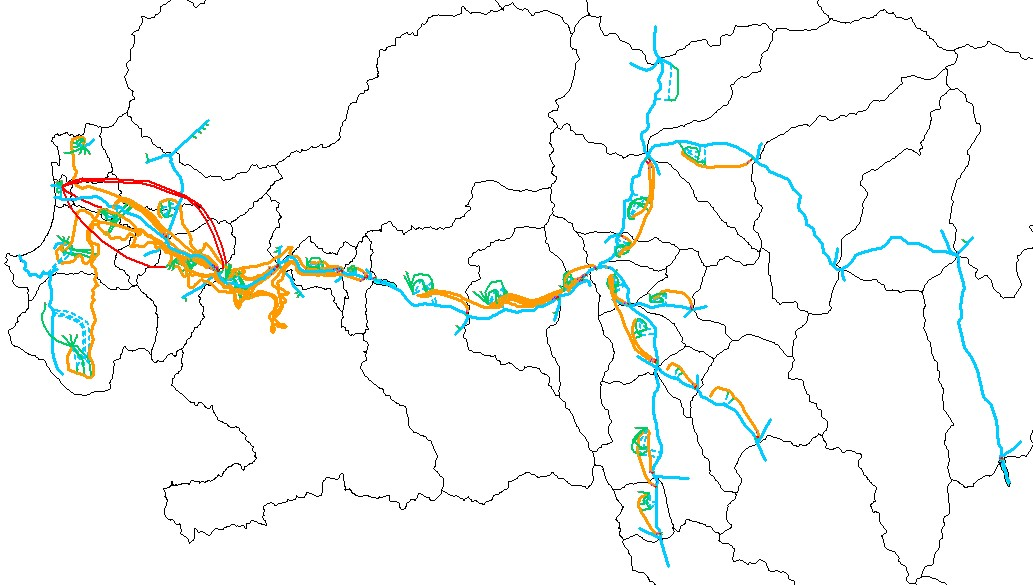
\includegraphics[width=\textwidth]{Figuras/Topologia_WEAP}}
\caption{Topología Modelo WEAP: Cuenca del río Elqui CRDP - PROMMRA}
\label{etiqueta_figura6}
\end{center}
\end{figure}

\subsubsection{Cauces Naturales}\bigskip

En la figura \ref{etiqueta_figura7} se observan los ríos y aportes naturales de la cuenca del Elqui, desarrolladas en base a SIG. El modelo contempla 10 ríos principales y 35 aportes naturales, correspondientes a quebrada, la nomenclatura usada para los aportes naturales hacen referencia a la zona donde se generan. En el cuadro \ref{tabla3} y cuadro \ref{tabla4} se listan las nombres correspondiente a cada río y aporte natural desarrollado en el modelo. Cada cauce natural, está ligado a un archivo de datos en formato .CSV que contiene la serie de caudales mensuales para la serie modelada. 
	
\begin{figure}[H]
\begin{center}
\fbox{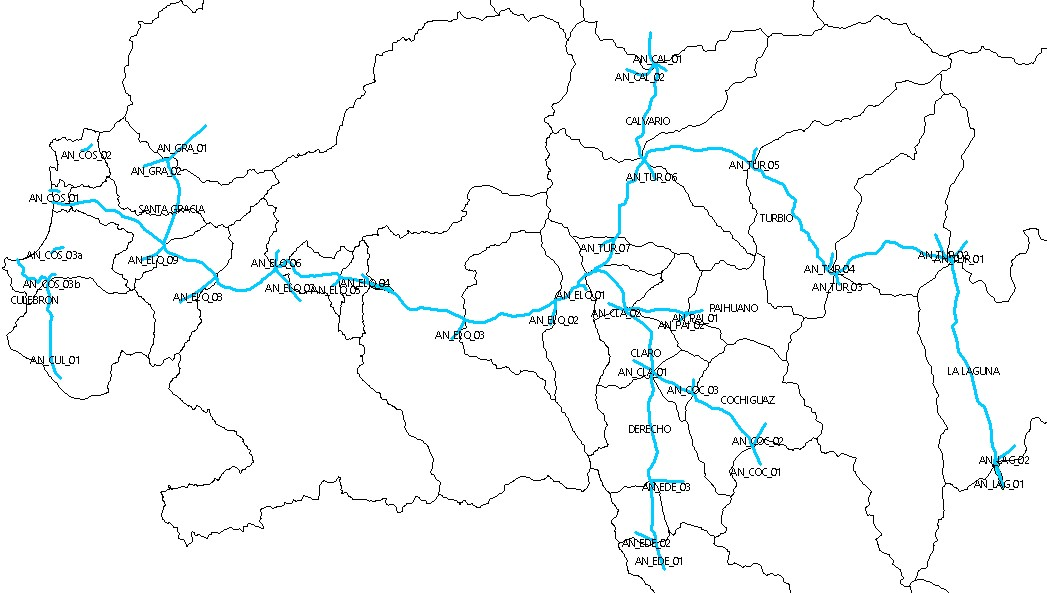
\includegraphics[width=\textwidth]{Figuras/CaucesNaturales}}
\caption{Modelo Cuenca del río Elqui CRDP - PROMMRA: Cauces naturales.}
\label{etiqueta_figura7}
\end{center}
\end{figure}


\begin{table}[H]
\centering
\caption{Nombre de los ríos esquematizados en el Modelo.}
\label{tabla3}
\begin{tabular}{@{}cl@{}}
\toprule
\textbf{Componente} & \multicolumn{1}{c}{\textbf{Nombre}} \\ \midrule
\multirow{10}{*}{Ríos} & LA LAGUNA \\
 & ESTERO DERECHO \\
 & COCHIGUAZ \\
 & PAIHUANO \\
 & CLARO \\
 & CALVARIO \\
 & TURBIO \\
 & ELQUI \\
 & SANTA GRACIA \\
 & CULEBRON \\ \midrule 
\end{tabular}
\end{table}

\begin{table}[H]
\centering
\caption{Nombre de los aportes naturales esquematizados en el Modelo}
\label{tabla4}
\begin{tabular}{@{}clll@{}}
\toprule
\textbf{Componente} & \multicolumn{1}{c}{\textbf{Nombre}} & \multicolumn{1}{c}{\textbf{}} & \multicolumn{1}{c}{\textbf{Nombre}} \\ \midrule
\multirow{18}{*}{\begin{tabular}[c]{@{}c@{}}Aportes\\   Naturales\end{tabular}} & AN\_EDE\_01 &  & AN\_TUR\_07 \\
 & AN\_EDE\_02 &  & AN\_ELQ\_01 \\
 & AN\_EDE\_03 &  & AN\_ELQ\_02 \\
 & AN\_COC\_01 &  & AN\_ELQ\_03 \\
 & AN\_COC\_02 &  & AN\_ELQ\_04 \\
 & AN\_COC\_03 &  & AN\_ELQ\_05 \\
 & AN\_PAI\_01 &  & AN\_ELQ\_06 \\
 & AN\_PAI\_02 &  & AN\_ELQ\_07 \\
 & AN\_CLA\_01 &  & AN\_ELQ\_08 \\
 & AN\_CLA\_02 &  & AN\_ELQ\_09 \\
 & AN\_LAG\_01 &  & AN\_GRA\_01 \\
 & AN\_LAG\_02 &  & AN\_GRA\_02 \\
 & AN\_TUR\_01 &  & AN\_CUL\_01 \\
 & AN\_TUR\_02 &  & AN\_COS\_01 \\
 & AN\_TUR\_03 &  & AN\_COS\_02 \\
 & AN\_TUR\_04 &  & AN\_CAL\_01 \\
 & AN\_TUR\_05 &  & AN\_CAL\_02 \\
 & AN\_TUR\_06 &  &  \\ \bottomrule
\end{tabular}
\end{table}

\subsubsection{Cauces Artificiales}\bigskip

En la figura  \ref{etiqueta_figura8} se observa la topología desarrollada para los cauces artificiales que componen el modelo Elqui. Cabe destacar, que estos cauces artificiales corresponde a agrupaciones de canales que comparten geográficamente un área determinada, con el objetivo de simplificar la calibración del modelo. Cada uno de estos cauces artificiales cuenta con respectivos número de acciones y el porcentaje de pérdidas en su conducción, las cuales son derivadas a acuíferos o como recuperaciones al río. \\

Por otra parte, estos cauces artificiales, se encuentran ligados a un nodo de demanda que permite el ingreso de agua por parte del río, en función a los derechos que estos posean y la disponibilidad hídrica existente, es decir, al desmarque asociado en cada una de las temporadas. \\

\begin{figure}[H]
\begin{center}
\fbox{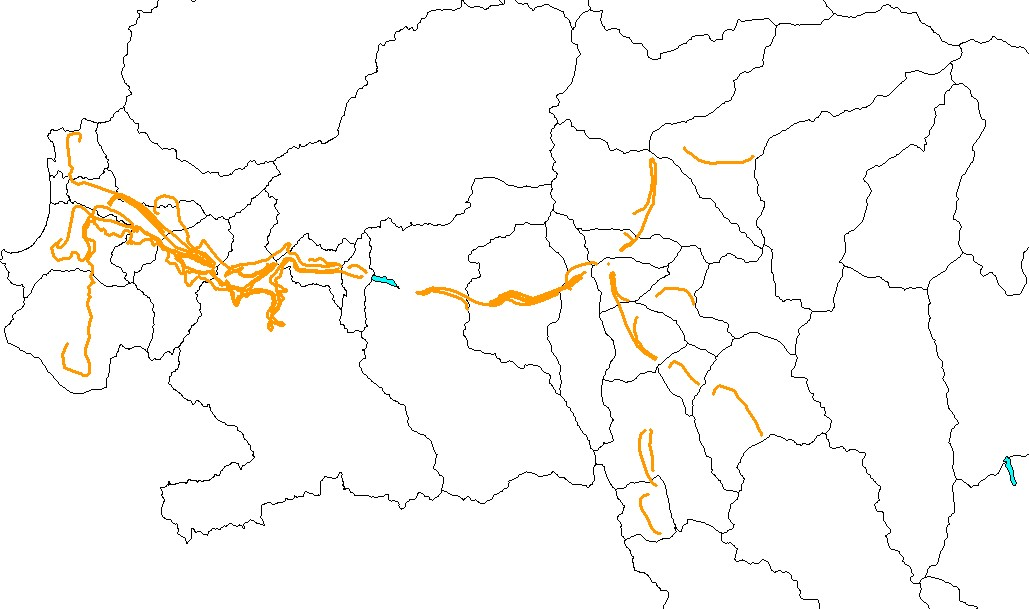
\includegraphics[width=\textwidth]{Figuras/CaucesArtificiales}}
\caption{Modelo Cuenca del río Elqui CRDP - PROMMRA: Cauces artificiales.}
\label{etiqueta_figura8}
\end{center}
\end{figure}

En total son 35 agrupaciones de canales o cauces artificiales creados para el modelo Elqui, donde 22 de ellos están ligados al río Elqui. Los respectivos nombres asignados a cada cauce artificial se detallan en el cuadro \ref{tabla5}. La nomenclatura designada tiene relación con el área o la subcuenca donde se encuentran ubicados la agrupación de canales.\\

\begin{table}[H]
\centering
\caption{Nombres de los cauces artificiales generados en el modelo.}
\label{tabla5}
\begin{tabular}{@{}cll@{}}
\toprule
\multicolumn{1}{c}{\textbf{Nombre del canal}} & \multicolumn{1}{c}{\textbf{Zona Asociada}} \\ \midrule
 CA\_EDE\_01 & Estero Derecho \\
 CA\_EDE\_02 & Estero Derecho \\
 CA\_EDE\_03 & Estero Derecho \\
 CA\_COC\_01 & Cochiguaz \\
 CA\_COC\_02 & Cochiguaz \\
 CA\_CLA\_01 & Río Claro \\
 CA\_CLA\_03 & Río Claro \\
 CA\_CLA\_02 & Río Claro \\
 CA\_PAI\_01 & Paihuano \\
 CA\_TUR\_01 & Río Turbio \\
 CA\_TUR\_02 & Río Turbio \\
 CA\_TUR\_03 & Río Turbio \\
 CA\_TUR\_04 & Río Turbio \\
 CA\_ELQ\_01 & Río Elqui \\
 CA\_ELQ\_02 & Río Elqui \\
 CA\_ELQ\_03 & Río Elqui \\
 CA\_ELQ\_04 & Río Elqui \\
 CA\_ELQ\_05 & Río Elqui \\
 CA\_ELQ\_06 & Río Elqui \\
 CA\_ELQ\_07 & Río Elqui \\
 CA\_ELQ\_08 & Río Elqui \\
 CA\_ELQ\_09 & Río Elqui \\
 CA\_ELQ\_10 & Río Elqui \\
 CA\_ELQ\_11 & Río Elqui \\
 CA\_ELQ\_12 & Río Elqui \\
 CA\_ELQ\_13 & Río Elqui \\
 CA\_ELQ\_14 & Río Elqui \\
 CA\_ELQ\_15 & Río Elqui \\
 CA\_ELQ\_16 & Río Elqui \\
 CA\_ELQ\_17 & Río Elqui \\
 CA\_ELQ\_18 & Río Elqui \\
 CA\_ELQ\_19 & Río Elqui \\
 CA\_ELQ\_20 & Río Elqui \\
 CA\_ELQ\_21 & Río Elqui \\
 CA\_ELQ\_26 & Río Elqui \\ \bottomrule
\end{tabular}
\end{table}


\subsubsection{Embalses}\bigskip

La cuenca del río Elqui cuenta con 2 obras de acumulación, el embalse La Laguna con 40 $Mm^3$ nominales, y el embalse Puclaro con 200 $Mm^3$. Ambos se crearon en el modelo, bajo las mismas características hidraúlicas respectivamente, además de su posicionamiento en la cuenca (Figura \ref{etiqueta_figura8}). Las extracciones mensuales de los embalses obedecen a un dato ingresado en el modelo mediante un archivo .csv. De esta manera, su operación esta ligado a lo que el dato asigne para distribuir, sin tomar en cuenta la demanda existente en su área de influencia.


\begin{figure}[H]
\begin{center}
\fbox{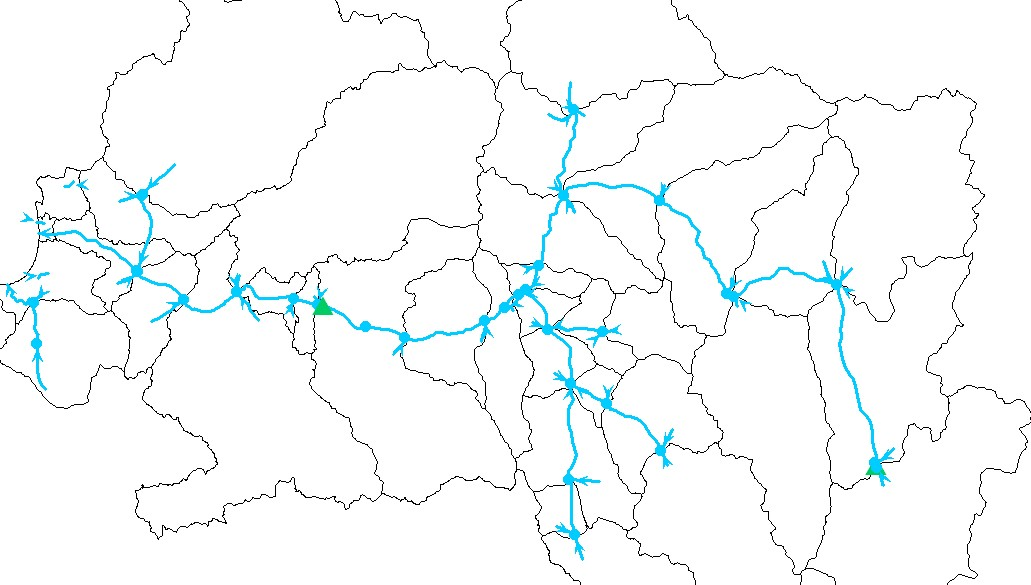
\includegraphics[width=\textwidth]{Figuras/EmbalsesWEAP}}
\caption{Modelo Cuenca del río Elqui CRDP - PROMMRA: Embalses.}
\label{etiqueta_figura8}
\end{center}
\end{figure}


\subsubsection{Acuíferos}\bigskip

Existen 22 acuíferos en el modelo, donde cada uno de ellos se configuró de acuerdo a su capacidad de almacenamiento, además de las recargas y extracciones que cada uno pueda tener según su área de influencia. Cabe destacar, que cada acuífero es una fuente hídrica para satisfacer las demandas que puedan tener asociadas, sin embargo, sus aguas son utilizadas sólo  cuando se hayan utilizado el total de los derechos de agua superficiales y sus demandas sigan insatisfechas. La disposición topológica de cada acuífero se observa en la figura \ref{etiqueta_figura9}

\begin{figure}[H]
\begin{center}
\fbox{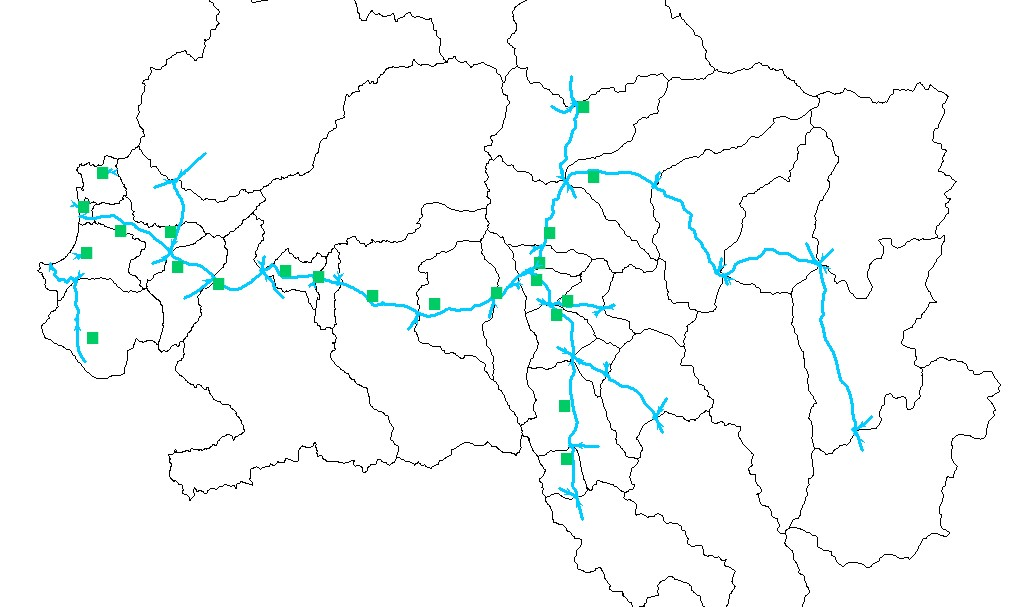
\includegraphics[width=\textwidth]{Figuras/AcuiferosWEAP}}
\caption{Modelo Cuenca del río Elqui CRDP - PROMMRA: Acuíferos.}
\label{etiqueta_figura9}
\end{center}
\end{figure}

La nomenclatura utilizada para cada acuífero está asociada a la zona de influencia que se encuentra asociada, esta se detalla en el cuadro \ref{tabla6}.\\

\begin{table}[H]
\centering
\caption{Nomenclatura de los acuíferos esquematizados en el Modelo.}
\label{tabla6}
\begin{tabular}{@{}cll@{}}
\toprule
\multicolumn{1}{c}{\textbf{Nombre del nodo}} & \multicolumn{1}{c}{\textbf{Zona Asociada}} \\ \midrule
  AC\_EDE\_01 & Estero Derecho \\
  AC\_EDE\_02 & Estero Derecho \\
  AC\_CLA\_01 & Río Claro \\
  AC\_PAI\_01 & Paihuano \\
  AC\_CLA\_02 & Río Claro \\
  AC\_TUR\_01 & Río Turbio \\
  AC\_CAL\_01 & Calvario \\
  AC\_TUR\_02 & Río Turbio \\
  AC\_TUR\_03 & Río Turbio \\
  AC\_ELQ\_01 & Río Elqui \\
  AC\_ELQ\_02 & Río Elqui \\
  AC\_ELQ\_03 & Río Elqui \\
  AC\_ELQ\_04 & Río Elqui \\
  AC\_ELQ\_05 & Río Elqui \\
  AC\_ELQ\_06 & Río Elqui \\
  AC\_ELQ\_07 & Río Elqui \\
  AC\_GRA\_01 & Río Elqui \\
  AC\_ELQ\_08 & Río Elqui \\
  AC\_COS\_01 & Zona Costera \\
  AC\_COS\_02 & Zona Costera \\
  AC\_COS\_03 & Zona Costera \\
  AC\_CUL\_01 & Pan de Azúcar \\ \bottomrule
\end{tabular}
\end{table}

\subsubsection{Sitios de Demanda}\bigskip

Los consumos de diferentes demandas productivas no agrícolas, son creados en el modelo mediante nodos llamados \textit{sitios de demanda}. Cada uno de ellos, representa una extracción de agua según el propósito productivo. Su configuración como demanda hídrica, esta desarrollada como consumo mensual en $m^3$ en base a los derechos que cada actividad cuente. En la figura \ref{etiqueta_figura10}, se observa la topología de los \textit{sitios de demanda} que fueron desarrollados para el modelo de la cuenca de Elqui, que en suman 40 nodos.\\
 

\begin{figure}[H]
\begin{center}
\fbox{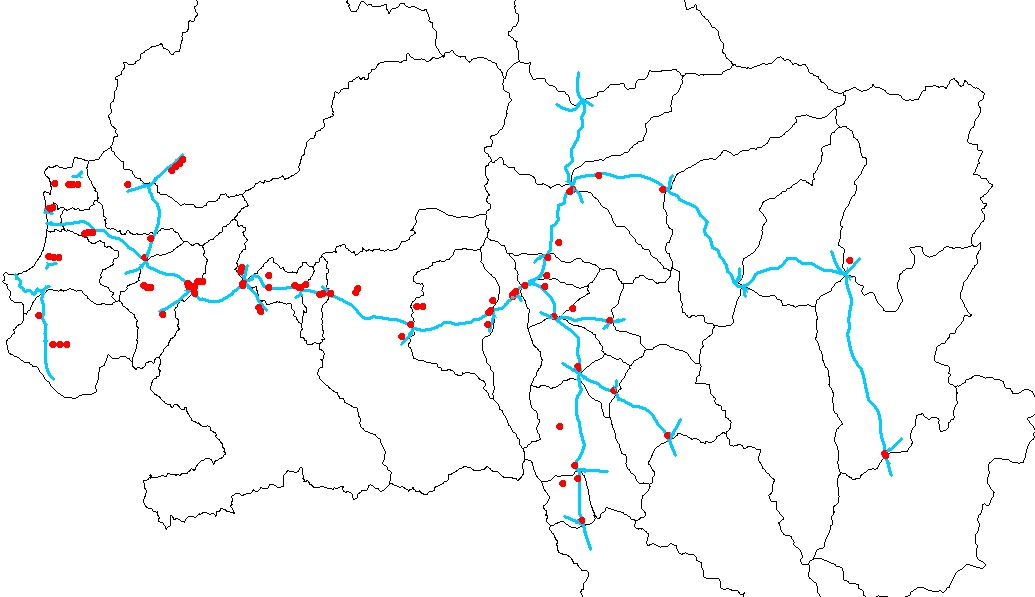
\includegraphics[width=\textwidth]{Figuras/SitiosDemanda}}
\caption{Modelo Cuenca del río Elqui CRDP - PROMMRA: Sitios de Demanda.}
\label{etiqueta_figura10}
\end{center}
\end{figure}

\begin{table}[H]
\centering
\caption{My caption}
\label{tabla7}
\begin{tabular}{@{}lllll@{}}
\toprule
\multicolumn{1}{c}{\textbf{Nombre del nodo}} & \multicolumn{1}{c}{\textbf{Tipo de Demanda}} &  & \multicolumn{1}{c}{\textbf{Nombre del Nodo}} & \multicolumn{1}{c}{\textbf{Tipo de Demanda}} \\ \midrule
AP\_AC\_ELQ\_02 & Agua Potable &  & I\_AC\_ELQ\_06 & Industria \\
AP\_AC\_ELQ\_03 & Agua Potable &  & I\_AC\_ELQ\_07 & Industria \\
AP\_AC\_ELQ\_05 & Agua Potable &  & M\_AC\_ELQ\_01 & Minería \\
AP\_AC\_ELQ\_06 & Agua Potable &  & M\_AC\_ELQ\_08 & Minería \\
AP\_AC\_ELQ\_07 & Agua Potable &  & M\_AC\_COS\_02 & Minería \\
AP\_AC\_ELQ\_08 & Agua Potable &  & M\_AC\_COS\_03 & Minería \\
AP\_AC\_GRA\_01 & Agua Potable &  & M\_AC\_COS\_01 & Minería \\
AP\_AC\_PAI\_01 & Agua Potable &  & M\_AC\_CUL\_01 & Minería \\
AP\_AC\_COS\_02 & Agua Potable &  & M\_AN\_ELQ\_06 & Minería \\
AP\_AC\_COS\_03 & Agua Potable &  & M\_AN\_ELQ\_07 & Minería \\
AP\_AC\_COS\_01 & Agua Potable &  & M\_AN\_GRA\_01 & Minería \\
AP\_AC\_CUL\_01 & Agua Potable &  & M\_AN\_TUR\_01 & Minería \\
AP\_AN\_GRA\_01 & Agua Potable &  & M\_AC\_ELQ\_06 & Minería \\
I\_AC\_ELQ\_02 & Industria &  & R\_AN\_ELQ\_02 & Riego \\
I\_AC\_ELQ\_08 & Industria &  & R\_AN\_ELQ\_03 & Riego \\
I\_AC\_COS\_02 & Industria &  & R\_AN\_ELQ\_06 & Riego \\
I\_AC\_COS\_03 & Industria &  & R\_AN\_ELQ\_07 & Riego \\
I\_AC\_COS\_01 & Industria &  & R\_AN\_ELQ\_08 & Riego \\
I\_AC\_CUL\_01 & Industria &  & R\_AN\_GRA\_01 & Riego \\
I\_AN\_GRA\_01 & Industria &  & R\_AN\_GRA\_02 & Riego \\ \bottomrule
\end{tabular}
\end{table}

\subsubsection{Sitios de Demanda Agrícola}\bigskip

El modelo contempla zonas de riego en las distintas áreas de la cuenca, cada una de estas se subdividen en zonas de riego de cultivos anuales y zonas de riego de cultivos frutales. Los datos que alimentan a estos nodos corresponden principalmente a superficie de riego ($ha$), tipo de cultivo y especie junto con su respectiva evapotranspiración, ademas del sistema de riego aplicado a su eficiencia. \\


\begin{figure}[H]
\begin{center}
\fbox{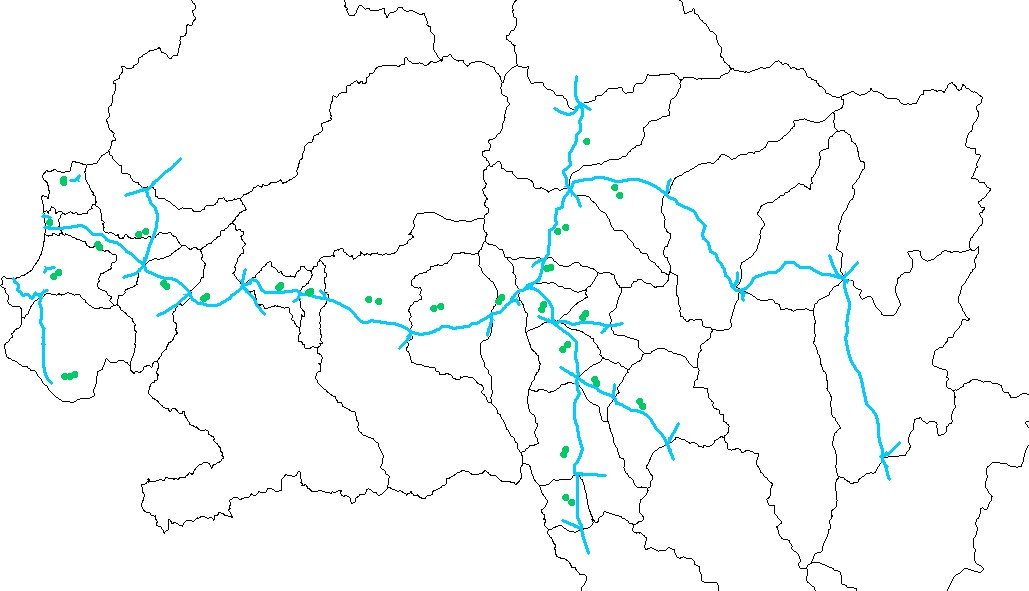
\includegraphics[width=\textwidth]{Figuras/DemandaAgricola}}
\caption{Modelo Cuenca del río Elqui CRDP - PROMMRA: Demanda Agrícola.}
\label{etiqueta_figura11}
\end{center}
\end{figure}

En el modelo existe un total de 46 nodos de demanda agrícola, donde su nomenclatura esta asociada al tipo de cultivo y la zona donde está ubicada. En el cuadro \ref{tabla8}, se presenta la lista de la nomenclatura utilizada para cada nodo y su respectiva zona de influencia.


\begin{table}[H]
\centering
\caption{Nomenclatura de las zonas de riego generadas en el Modelo.}
\label{tabla8}
\begin{tabular}{@{}lllll@{}}
\toprule
\multicolumn{1}{c}{\textbf{Nombre del nodo}} & \multicolumn{1}{c}{\textbf{Zona Asociada}} & \multicolumn{1}{c}{\textbf{}} & \multicolumn{1}{c}{\textbf{Nombre del Nodo}} & \multicolumn{1}{c}{\textbf{Zona Asociada}} \\ \midrule
ZR\_EDE\_01FRU & Estero Derecho &  & ZR\_ELQ\_02ANU & Río Elqui \\
ZR\_EDE\_02FRU & Estero Derecho &  & ZR\_ELQ\_03FRU & Río Elqui \\
ZR\_EDE\_01ANU & Estero Derecho &  & ZR\_ELQ\_03ANU & Río Elqui \\
ZR\_EDE\_02ANU & Estero Derecho &  & ZR\_ELQ\_04FRU & Río Elqui \\
ZR\_COC\_01FRU & Cochiguaz &  & ZR\_ELQ\_04ANU & Río Elqui \\
ZR\_COC\_02FRU & Cochiguaz &  & ZR\_ELQ\_05FRU & Río Elqui \\
ZR\_COC\_02ANU & Cochiguaz &  & ZR\_ELQ\_05ANU & Río Elqui \\
ZR\_CLA\_01FRU & Río Claro &  & ZR\_ELQ\_06FRU & Río Elqui \\
ZR\_CLA\_01ANU & Río Claro &  & ZR\_ELQ\_06ANU & Río Elqui \\
ZR\_PAI\_01FRU & Paihuano &  & ZR\_ELQ\_07FRU & Río Elqui \\
ZR\_PAI\_01ANU & Paihuano &  & ZR\_ELQ\_07ANU & Río Elqui \\
ZR\_CLA\_02FRU & Río Claro &  & ZR\_GRA\_01FRU & Santa Gracia \\
ZR\_CLA\_02ANU & Río Claro &  & ZR\_GRA\_01ANU & Santa Gracia \\
ZR\_TUR\_01FRU & Río Turbio &  & ZR\_ELQ\_08FRU & Río Elqui \\
ZR\_TUR\_01ANU & Río Turbio &  & ZR\_ELQ\_08ANU & Río Elqui \\
ZR\_CAL\_01FRU & Calvario &  & ZR\_COS\_01ANU & Zona Costera \\
ZR\_TUR\_02FRU & Río Turbio &  & ZR\_COS\_02FRU & Zona Costera \\
ZR\_TUR\_02ANU & Río Turbio &  & ZR\_COS\_03FRU & Zona Costera \\
ZR\_TUR\_03FRU & Río Turbio &  & ZR\_COS\_03ANU & Zona Costera \\
ZR\_TUR\_03ANU & Río Turbio &  & ZR\_CUL\_01FRU & Pan de Azúcar \\
ZR\_ELQ\_01FRU & Río Elqui &  & ZR\_CUL\_01ANU & Pan de Azúcar \\
ZR\_ELQ\_01ANU & Río Elqui &  & ZR\_CUL\_01OTR & Pan de Azúcar \\
ZR\_ELQ\_02FRU & Río Elqui &  & ZR\_COC\_01ANU & Cochiguaz \\ \bottomrule
\end{tabular}
\end{table}


		\subsection{Actualización del modelo Elqui}\bigskip
		
Para hacer operativo el modelo WEAP de la cuenca del río Elqui de acuerdo al funcionamiento que históricamente la JVRE ha trabajado y el posterior planteamiento de una regla operacional para la distribución del recurso hídrico, se debió hacer ajustes de actualización de datos para darle vigencia al modelo, además de configuraciones en la temporada hídrica, y en la forma que operan los embalses dentro del modelo. A continuación se describen las actualizaciones y modificaciones realizadas en las temáticas antes mencionadas.\\
		
			\subsubsection{Temporada Hídrica JVRE}		
		
		El modelo establecía que la temporada comenzara en el mes de abril y termina en el mes de marzo del siguiente año. Sin embargo, la JVRE trabaja sus temporadas hídricas en base a la planificación y la asignación desde el mes de septiembre hasta agosto del siguiente año. A raíz de ello, se cambió la configuración de la temporada en el modelo con la configuración Septiembre - Agosto, lo que contempló ajustar los datos de entrada para las variables que componen los nodos de demanda, tanto agrícola como de otros usos, en los meses que corresponde de acuerdo al cambio de temporada.\\
		
			\subsubsection{Operación de los embalse en el modelo}		
		
		Un punto importante que se modificó en el modelo, fue la operatividad de los embalses La Laguna y Puclaro, ya que estos distribuían el agua (efluentes), mediante datos mensuales que estaban alojados en un archivo \textit{.CSV}. Es decir, cada mes recurría a un dato para asignar cuanta agua iba distribuir en el mes correspondiente. Esta metodología, no permitía regular al propio embalse su asignación en función de la demanda que existiera bajo su área de influencia, si no mas bien, estaba sujeto a un dato ya previsto. \\
		
		
		
		
		
		
		
		
		
		\subsubsection{Incorporación Regla Operacional JVRE}\bigskip
			
		\subsection{Calibración y Validación del modelo Elqui}
		

 





\begin{itemize}
\item Para realizar interlineado entre párrafos se utiliza \verb!\\!.
\item Para \textbf{escribir en negrita}: \verb!\textbf{texto}!.
\item Para \textit{escribir en cursiva}: \verb!\textbit{texto}!.
\item Para \textit{\textbf{escribir en negrita y cursiva}}: \verb!\textit{\textbf{texto}}! (por lo tanto se pueden anidar los comandos).
\item Para crear una sección: \verb!\section{nombre}!.
\item Para crear una subsección: \verb!\subsection{nombre}!.
\item Para crear una subsubsección: \verb!\subsubsection{nombre}!.
\item Una lista como la actual se crea indicando donde comienza:\\
\verb!\begin{itemize}!\\
Cada ítem se debe ir agregando:\\
\verb!\item! un ítem cualquiera\\
Para cerrar la lista:\\
\verb!\end{itemize}!\\
\item Para cambiar el tamaño de la letra hay muchas opciones, una de ellas es \verb!\scriptsize{texto}! para obtener \scriptsize{un tamaño como este}\normalsize{.} % se bugea el tamaño de texto en listas
\item También se puede escribir en formato máquina de escribir para denotar código u otra cosa que requiera una fuente diferente: \verb!\texttt{texto}! y el \texttt{resultado será así}.
\end{itemize}

Para más información de formato y afines, visitar los sitios web \href{https://es.sharelatex.com/learn}{Share\LaTeX} y \href{https://en.wikibooks.org/wiki/LaTeX}{Wikibooks}.\\

\section{Citas\\}

En el caso de las citas,es algo más complicado de realizar. Primero, hay que descargar e instalar el paquete \texttt{flexbib} para poder personalizar bibliografías en español ya que \LaTeX por defecto compila las bibliografías en inglés (el vínculo de descarga se encuentra en la línea 9 del presente documento). De igual manera de pueden citar los documentos y añadirlos a la bibliografía, pero estarán con el formato en Inglés. Luego, hay que crear una base de datos en Zotero (recomendado) mediante los siguientes pasos:\\

\begin{figure}[!h]
\begin{center}
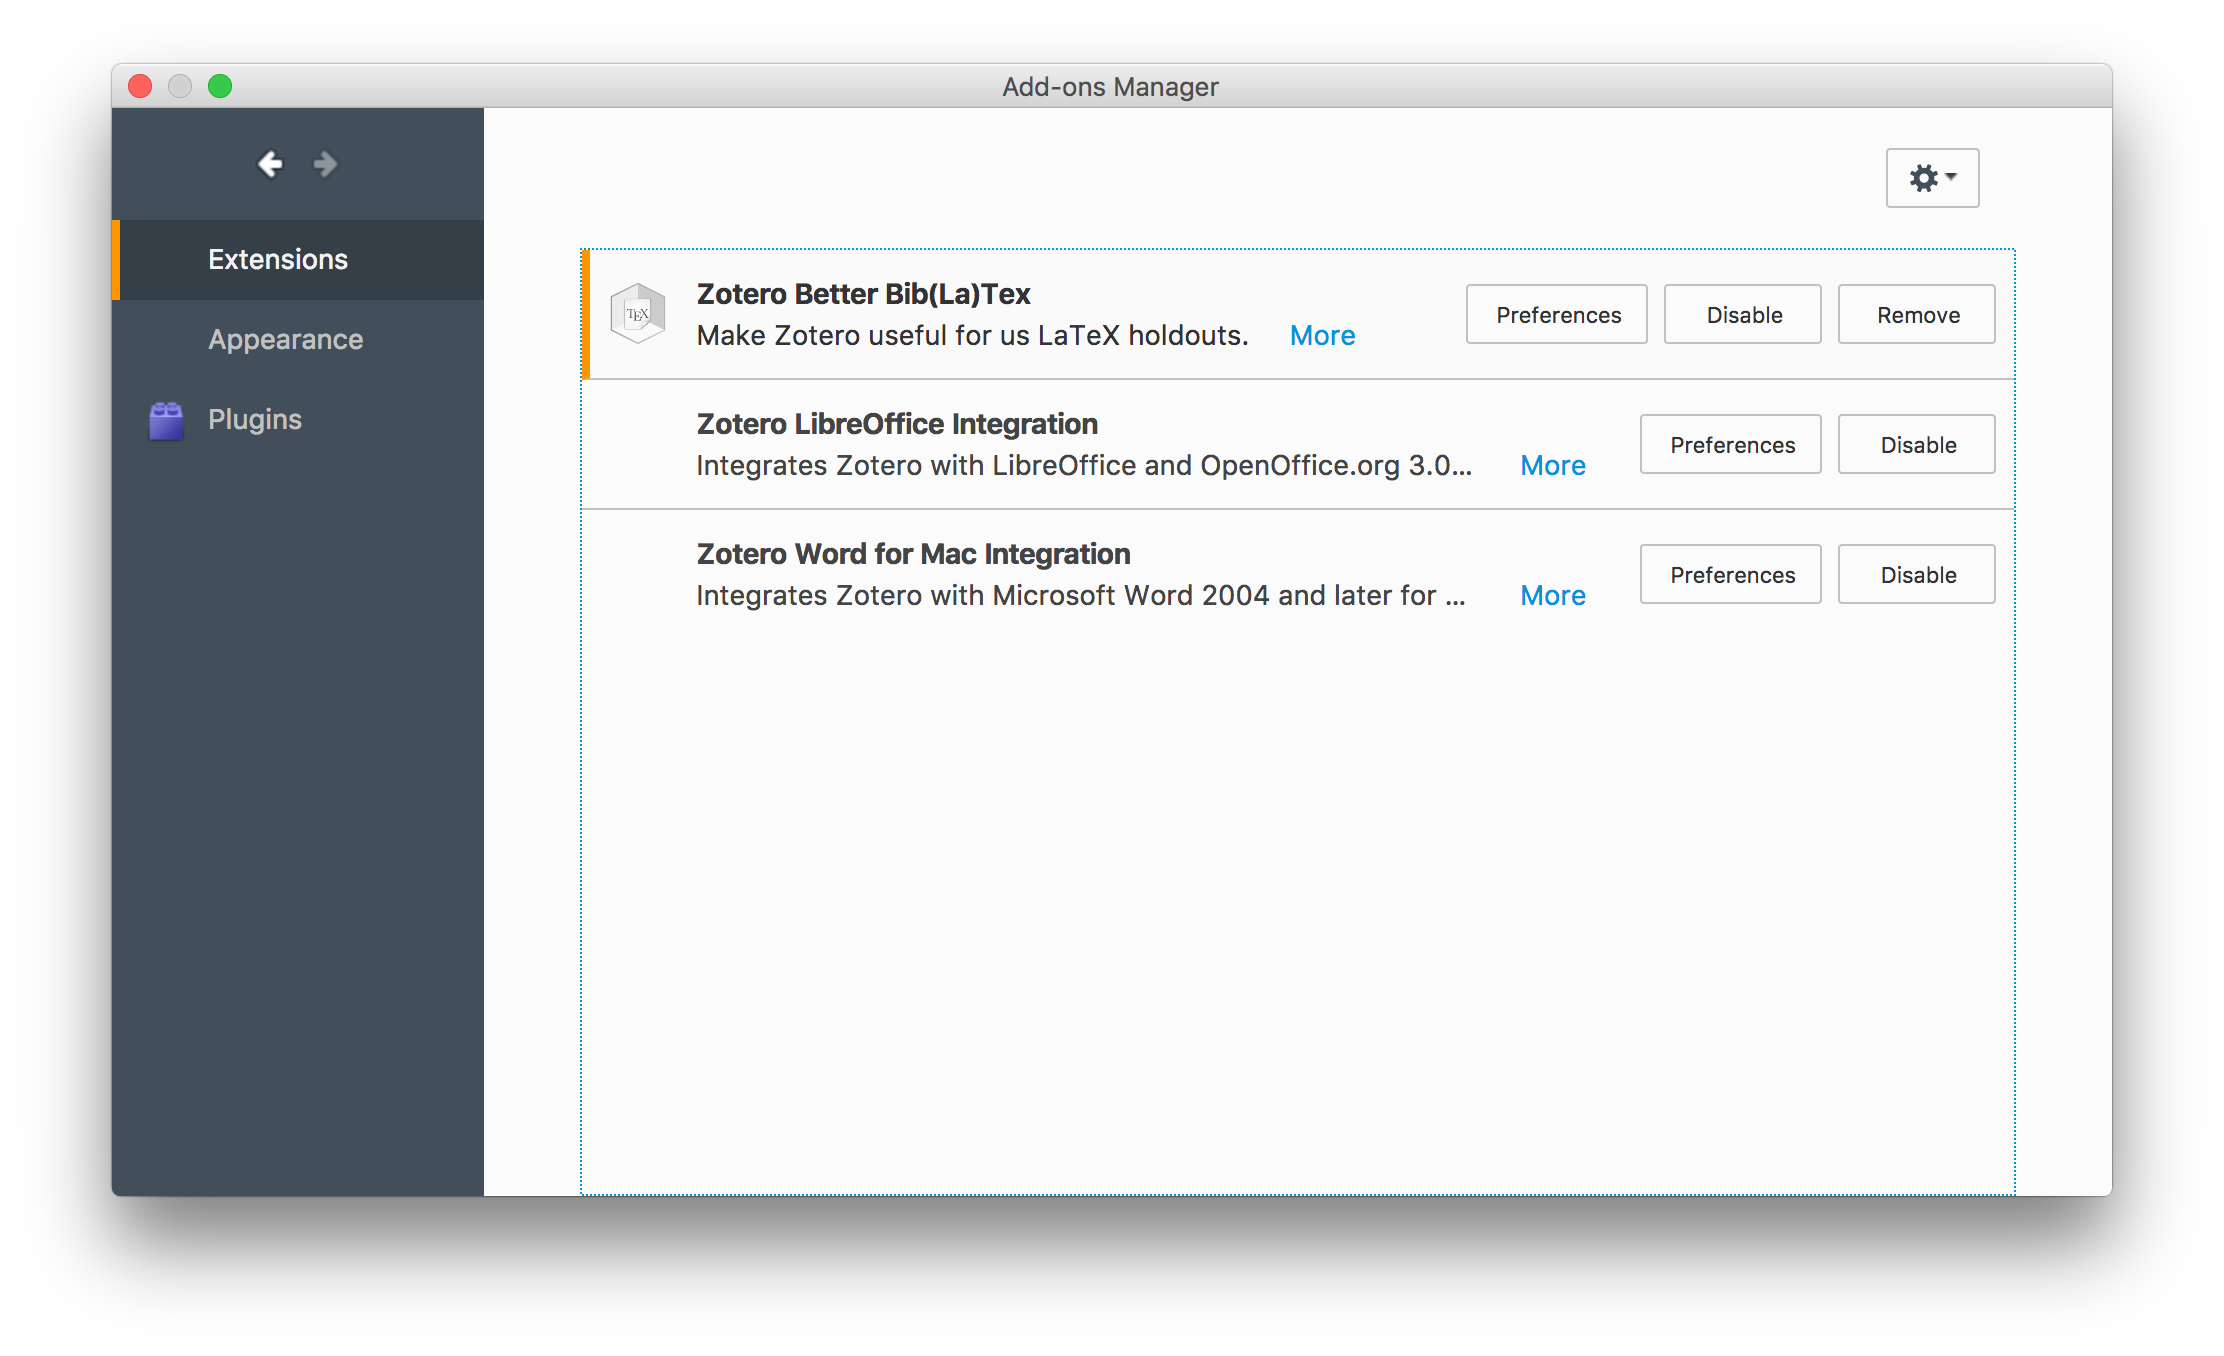
\includegraphics[width=\textwidth]{Figuras/plugins_zotero.png}
\caption{Installar Zotero y los plugins necesarios (especialmente el de flexbib).}
\label{etiqueta_figura1}
\end{center}
\end{figure}

\begin{figure}[!h]
\begin{center}
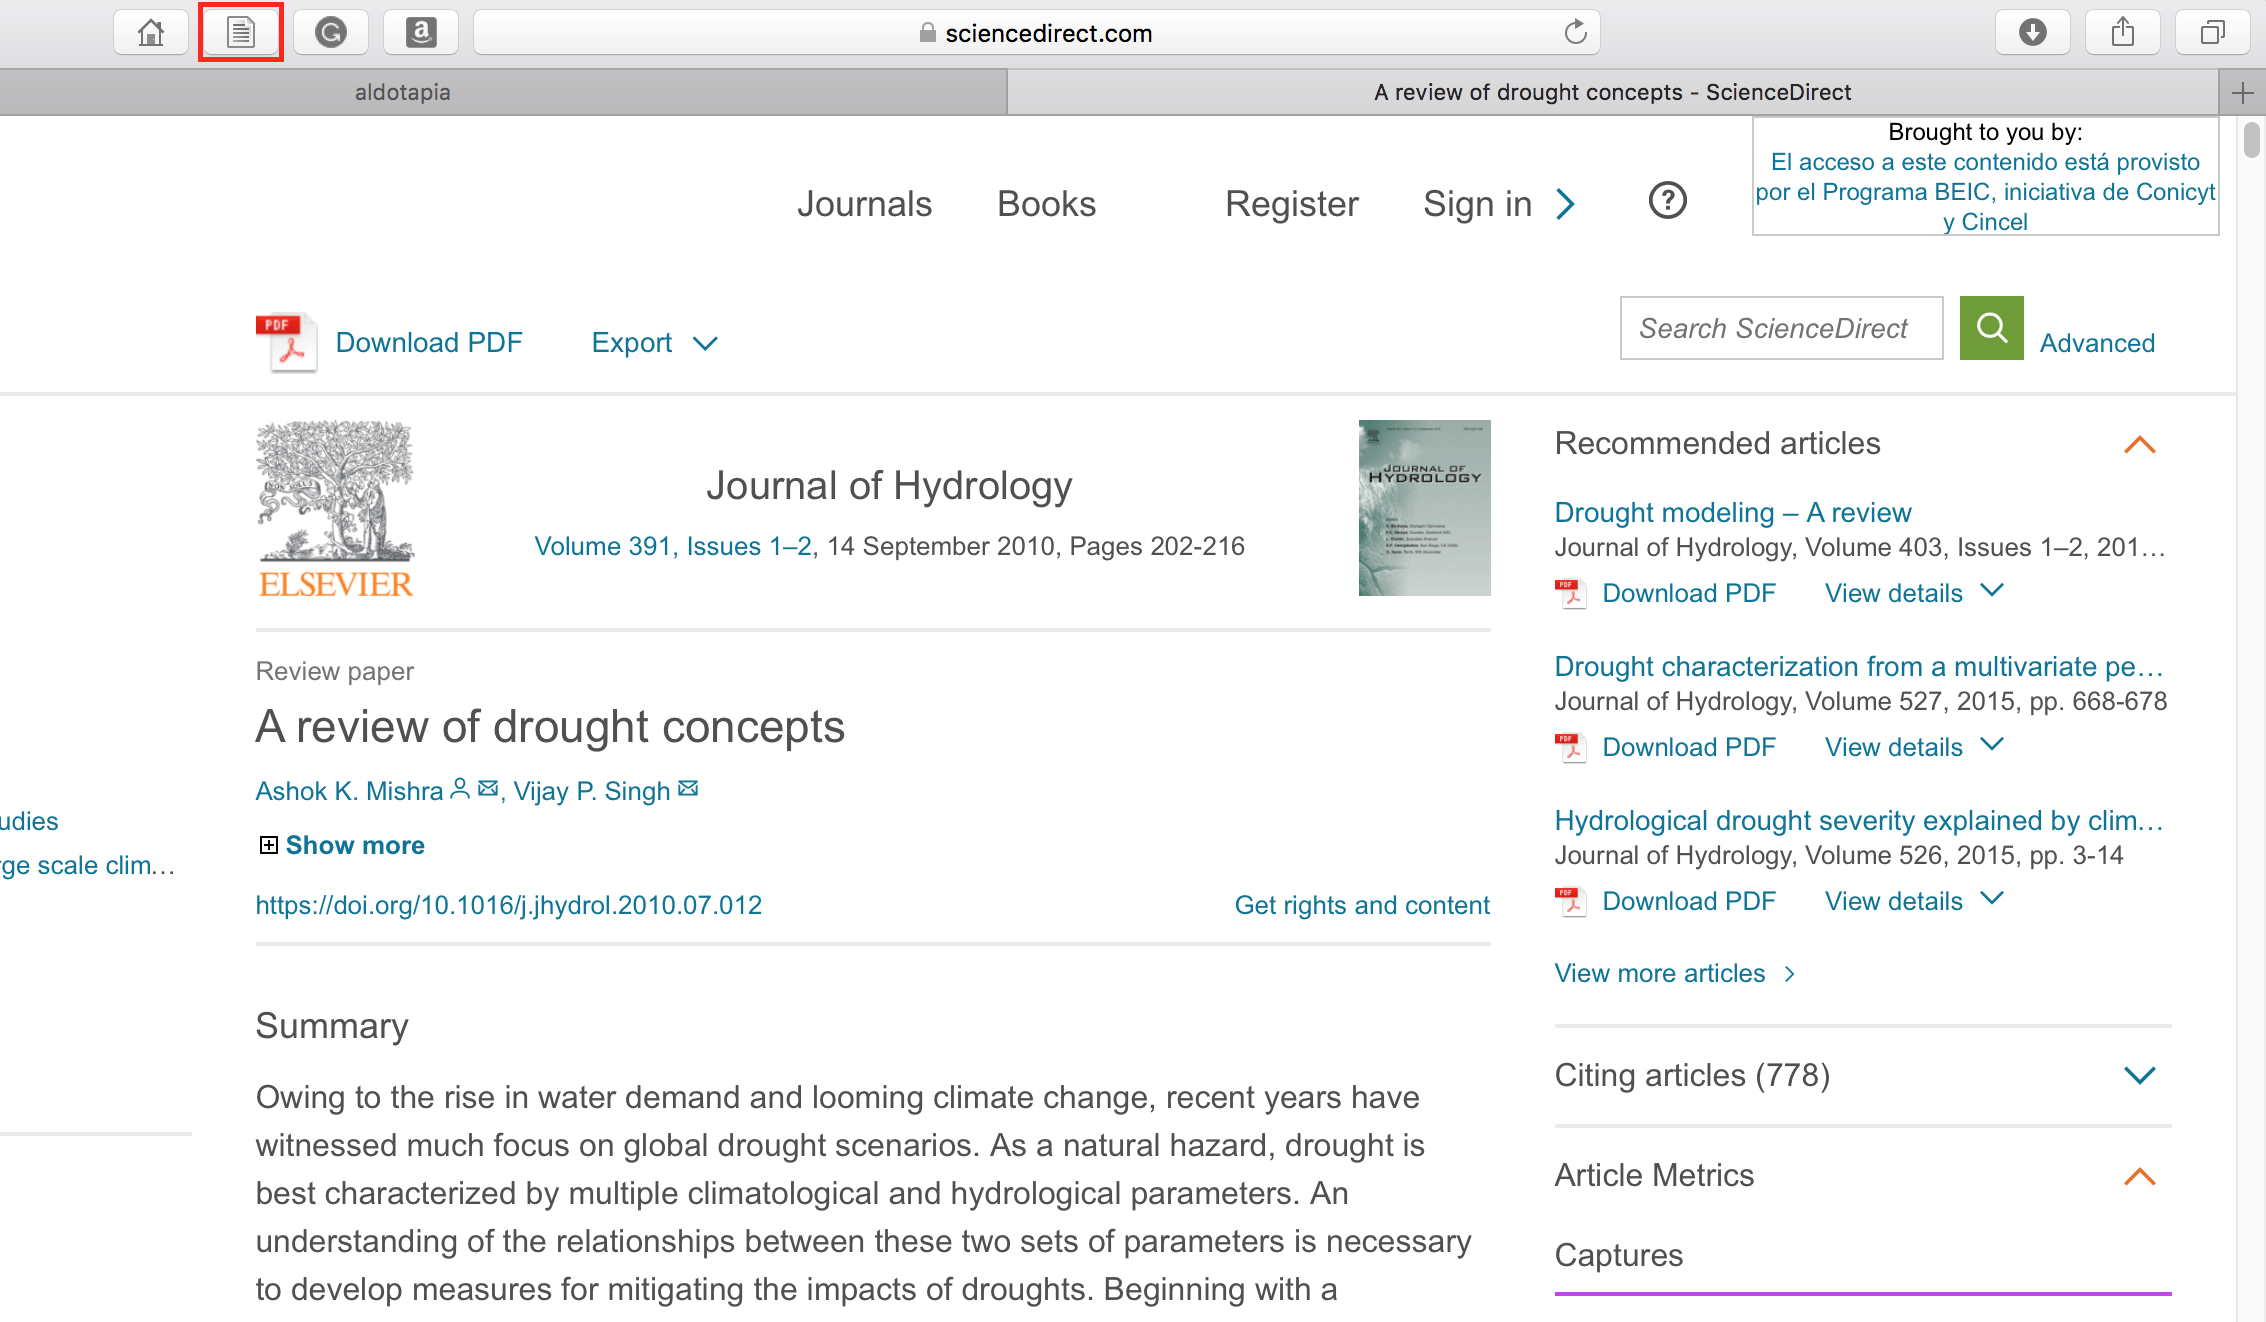
\includegraphics[width=\textwidth]{Figuras/zotero_web.png}
\caption{Clickear el ícono de Zotero para guardar cita}
\label{etiqueta_figura2}
\end{center}
\end{figure}

\begin{figure}[!h]
\begin{center}
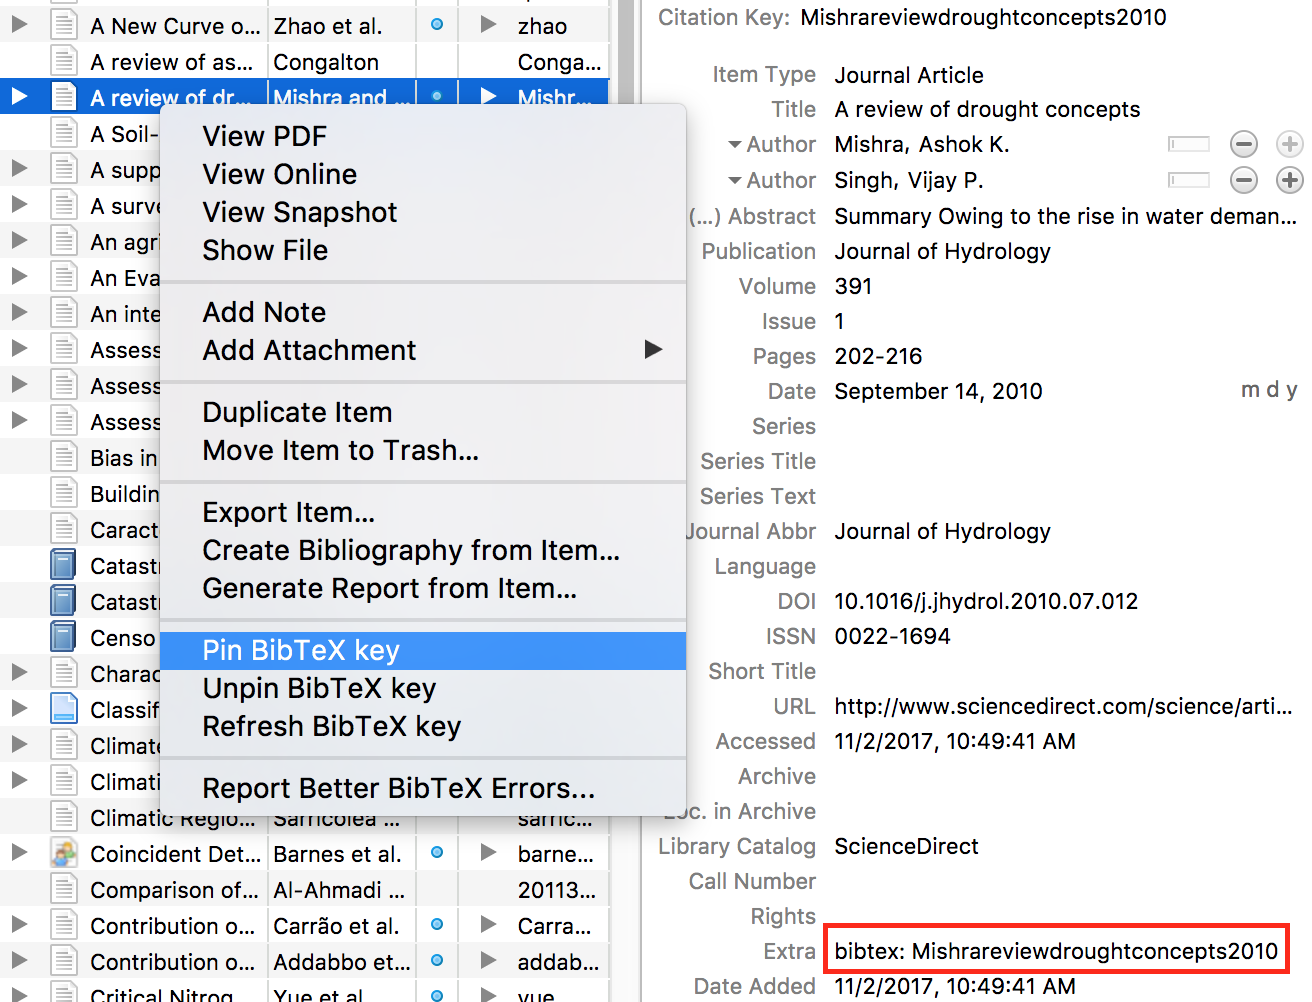
\includegraphics[width=\textwidth]{Figuras/zotero_pin.png}
\caption{Crear un pip de bibtex con la cita}
\label{etiqueta_figura3}
\end{center}
\end{figure}

\begin{figure}[!h]
\begin{center}
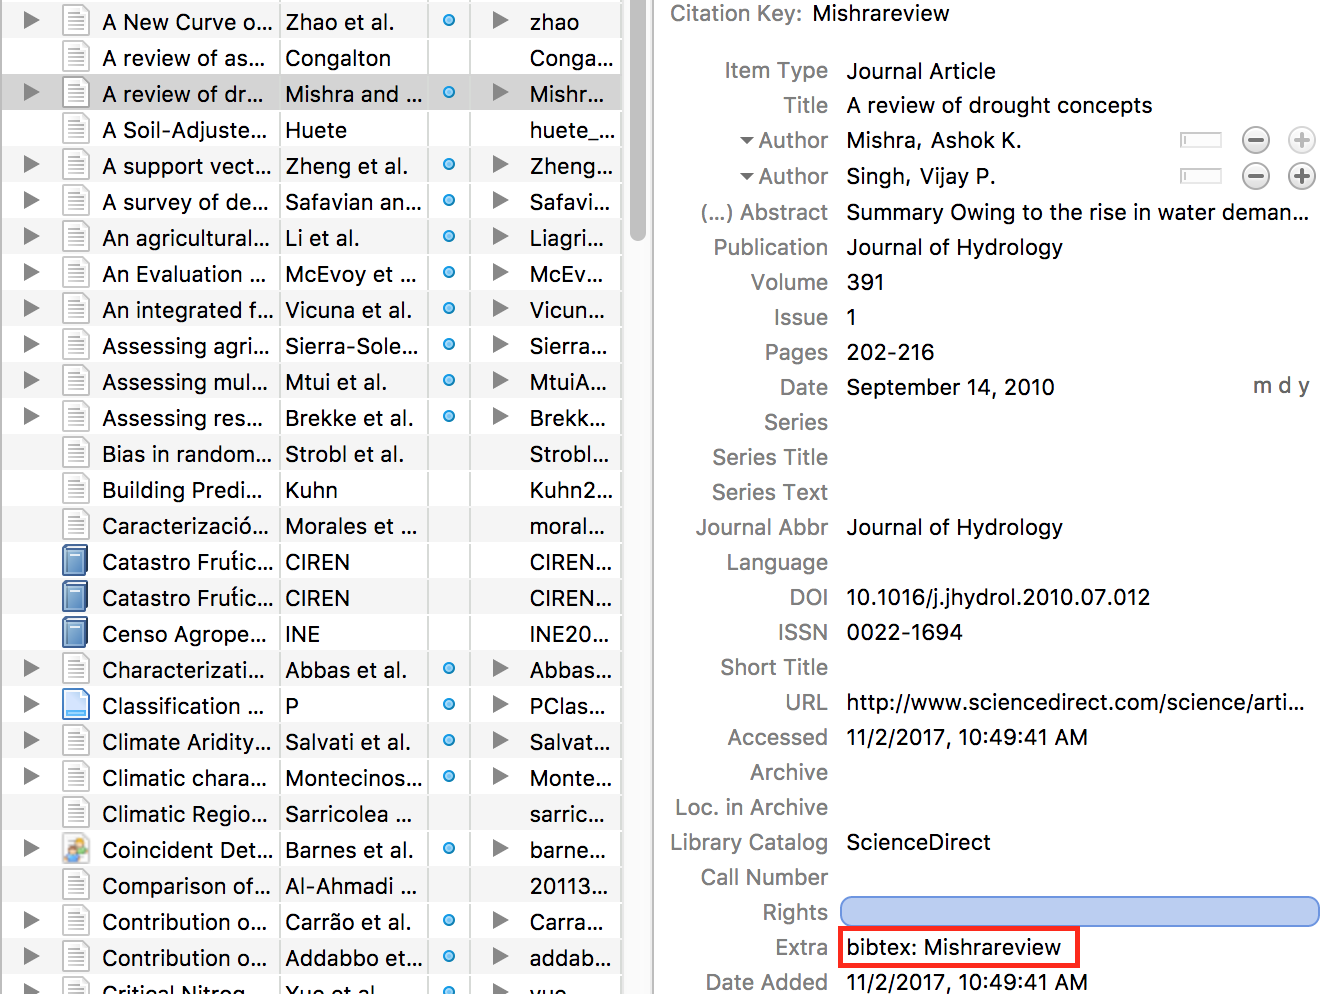
\includegraphics[width=\textwidth]{Figuras/zotero_pin2.png}
\caption{Modificar el pin si se requiere para facilitar la llamada en el documento}
\label{etiqueta_figura4}
\end{center}
\end{figure}

\begin{figure}[!h]
\begin{center}
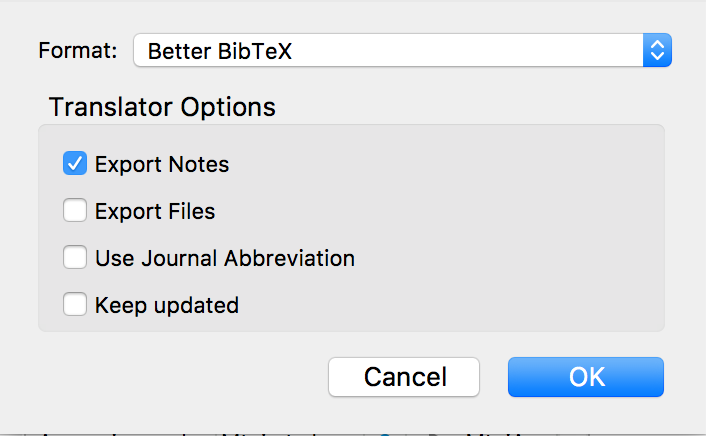
\includegraphics[width=\textwidth]{Figuras/better.png}
\caption{Exportar biblioteca como Better BibTex y guardarla en el mismo lugar donde está almacenado el archivo \texttt{nombre.tex}}
\label{etiqueta_figura5}
\end{center}
\end{figure}

\clearpage

Luego, llamar la cita en base al pin asignado, que en este caso es \verb!Mishrareview! con las funciones \verb!\cite{}! o \verb!\citep{}!. La primera es para citar con mención en el párrafo - como si \cite{Mishrareview} dijo algo - y la segunda; para citar con paréntesis \citep{Mishrareview}. Si se colocan comas entre los corchete para citar a una o más personas - como \verb!\citep{Mishrareview,huete1988}! - el resultado será una cita formateada con separadores \citep{Mishrareview,huete1988}.\\

\subsection{Información importante acerca de las citas\\}

XeLaTeX no compila la bibliografía automáticamente... La elección de este compilador es sólo por el uso de Century Gothic como fuente. Por lo tanto hay que compilar varias primero por XeLaTex, luego por BibTex (para crear la bibliografía), luego nuevamente por XeLaTex (aparecerá la bibliografía, pero las citas estarán con ?) y finalmente una última vez por XeLaTex y todo se compilará a la perfección. Para ello, he ocupado TeXShop para compilar.\\

\textbf{Información importante}: al utilizar RStudio para compilar los documentos, no es necesario seguir los pasos mencionados anteriormente. Sólo se utiliza el ícono \textit{Compile PDF} y el documento quedará correctamente compilado.

\section{Tablas\\}

Lo más sencillo para crear tablas es visitar el sitio web \href{https://www.tablesgenerator.com/latex_tables}{Tables Generator}. Sólo crean la tabla en excel, csv o otro formato. La cargan en el menu desplegable \verb!file! (Figura \ref{tabla1}) y copian el resultado que se obtiene (Figura \ref{tabla2}):

\begin{figure}[!h]
\begin{center}
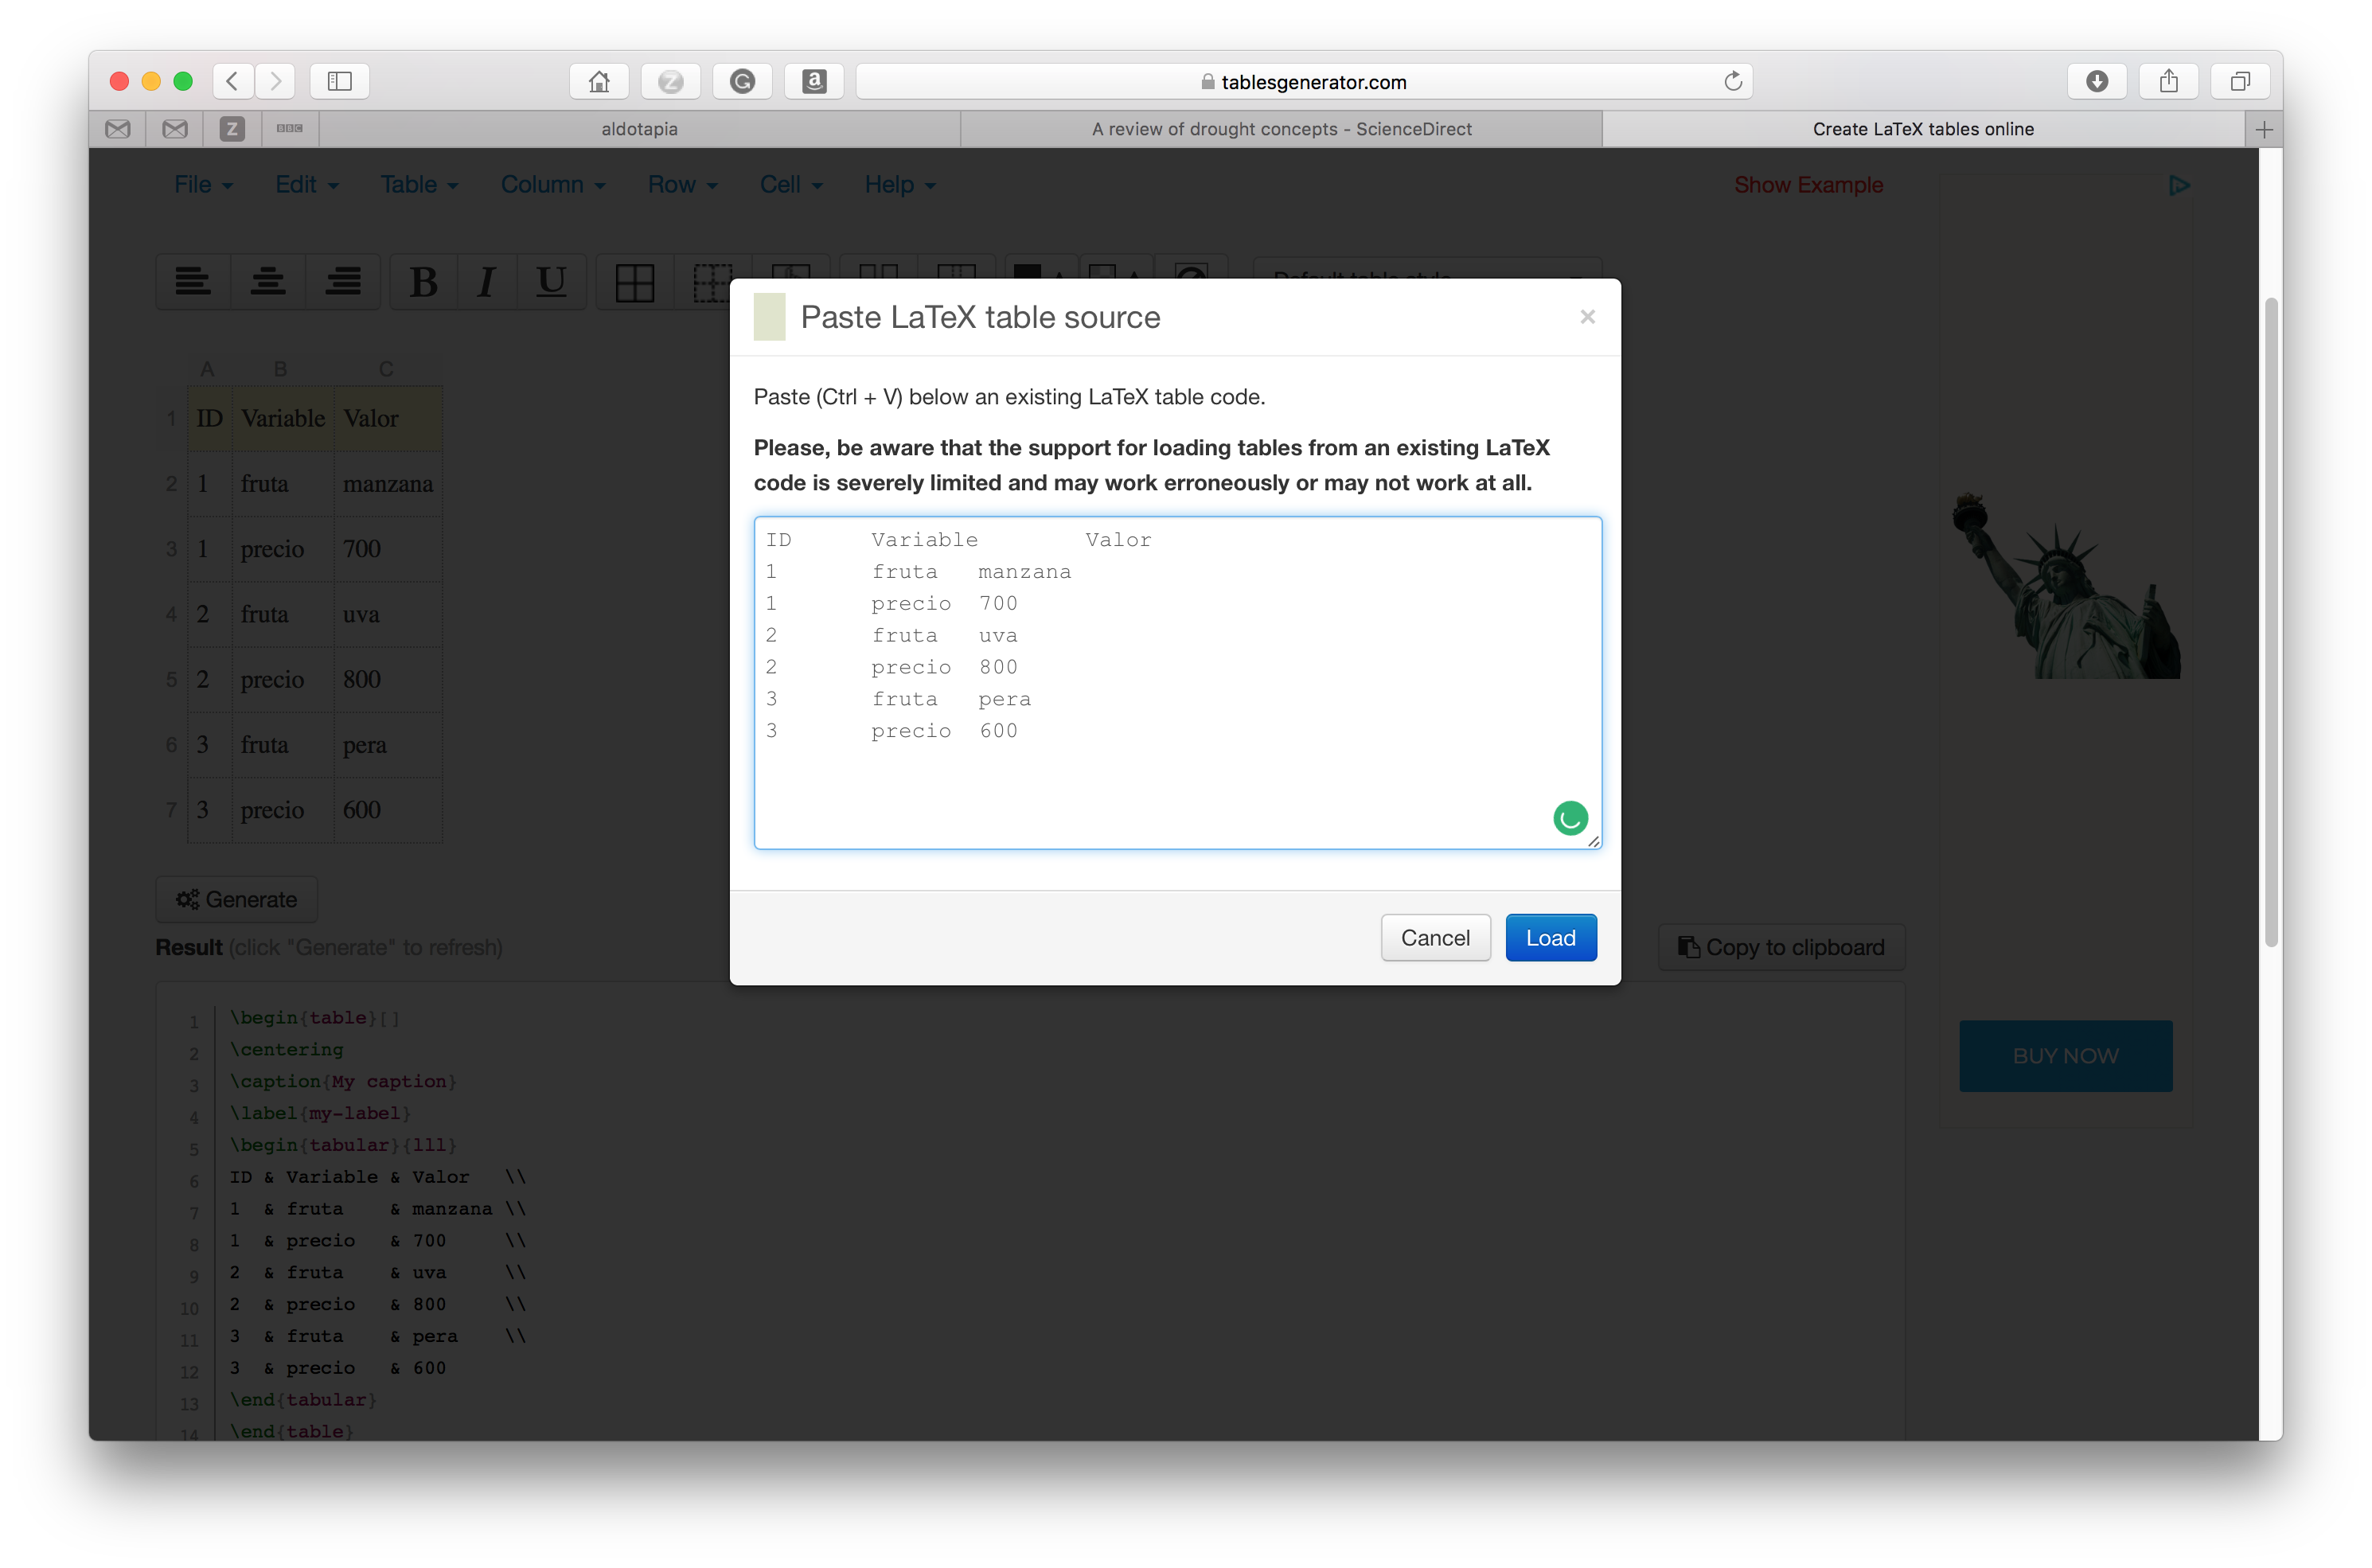
\includegraphics[width=\textwidth]{Figuras/tabla1.png}
\caption{Pegado de la tabla}
\label{tabla1}
\end{center}
\end{figure}

\begin{figure}[!h]
\begin{center}
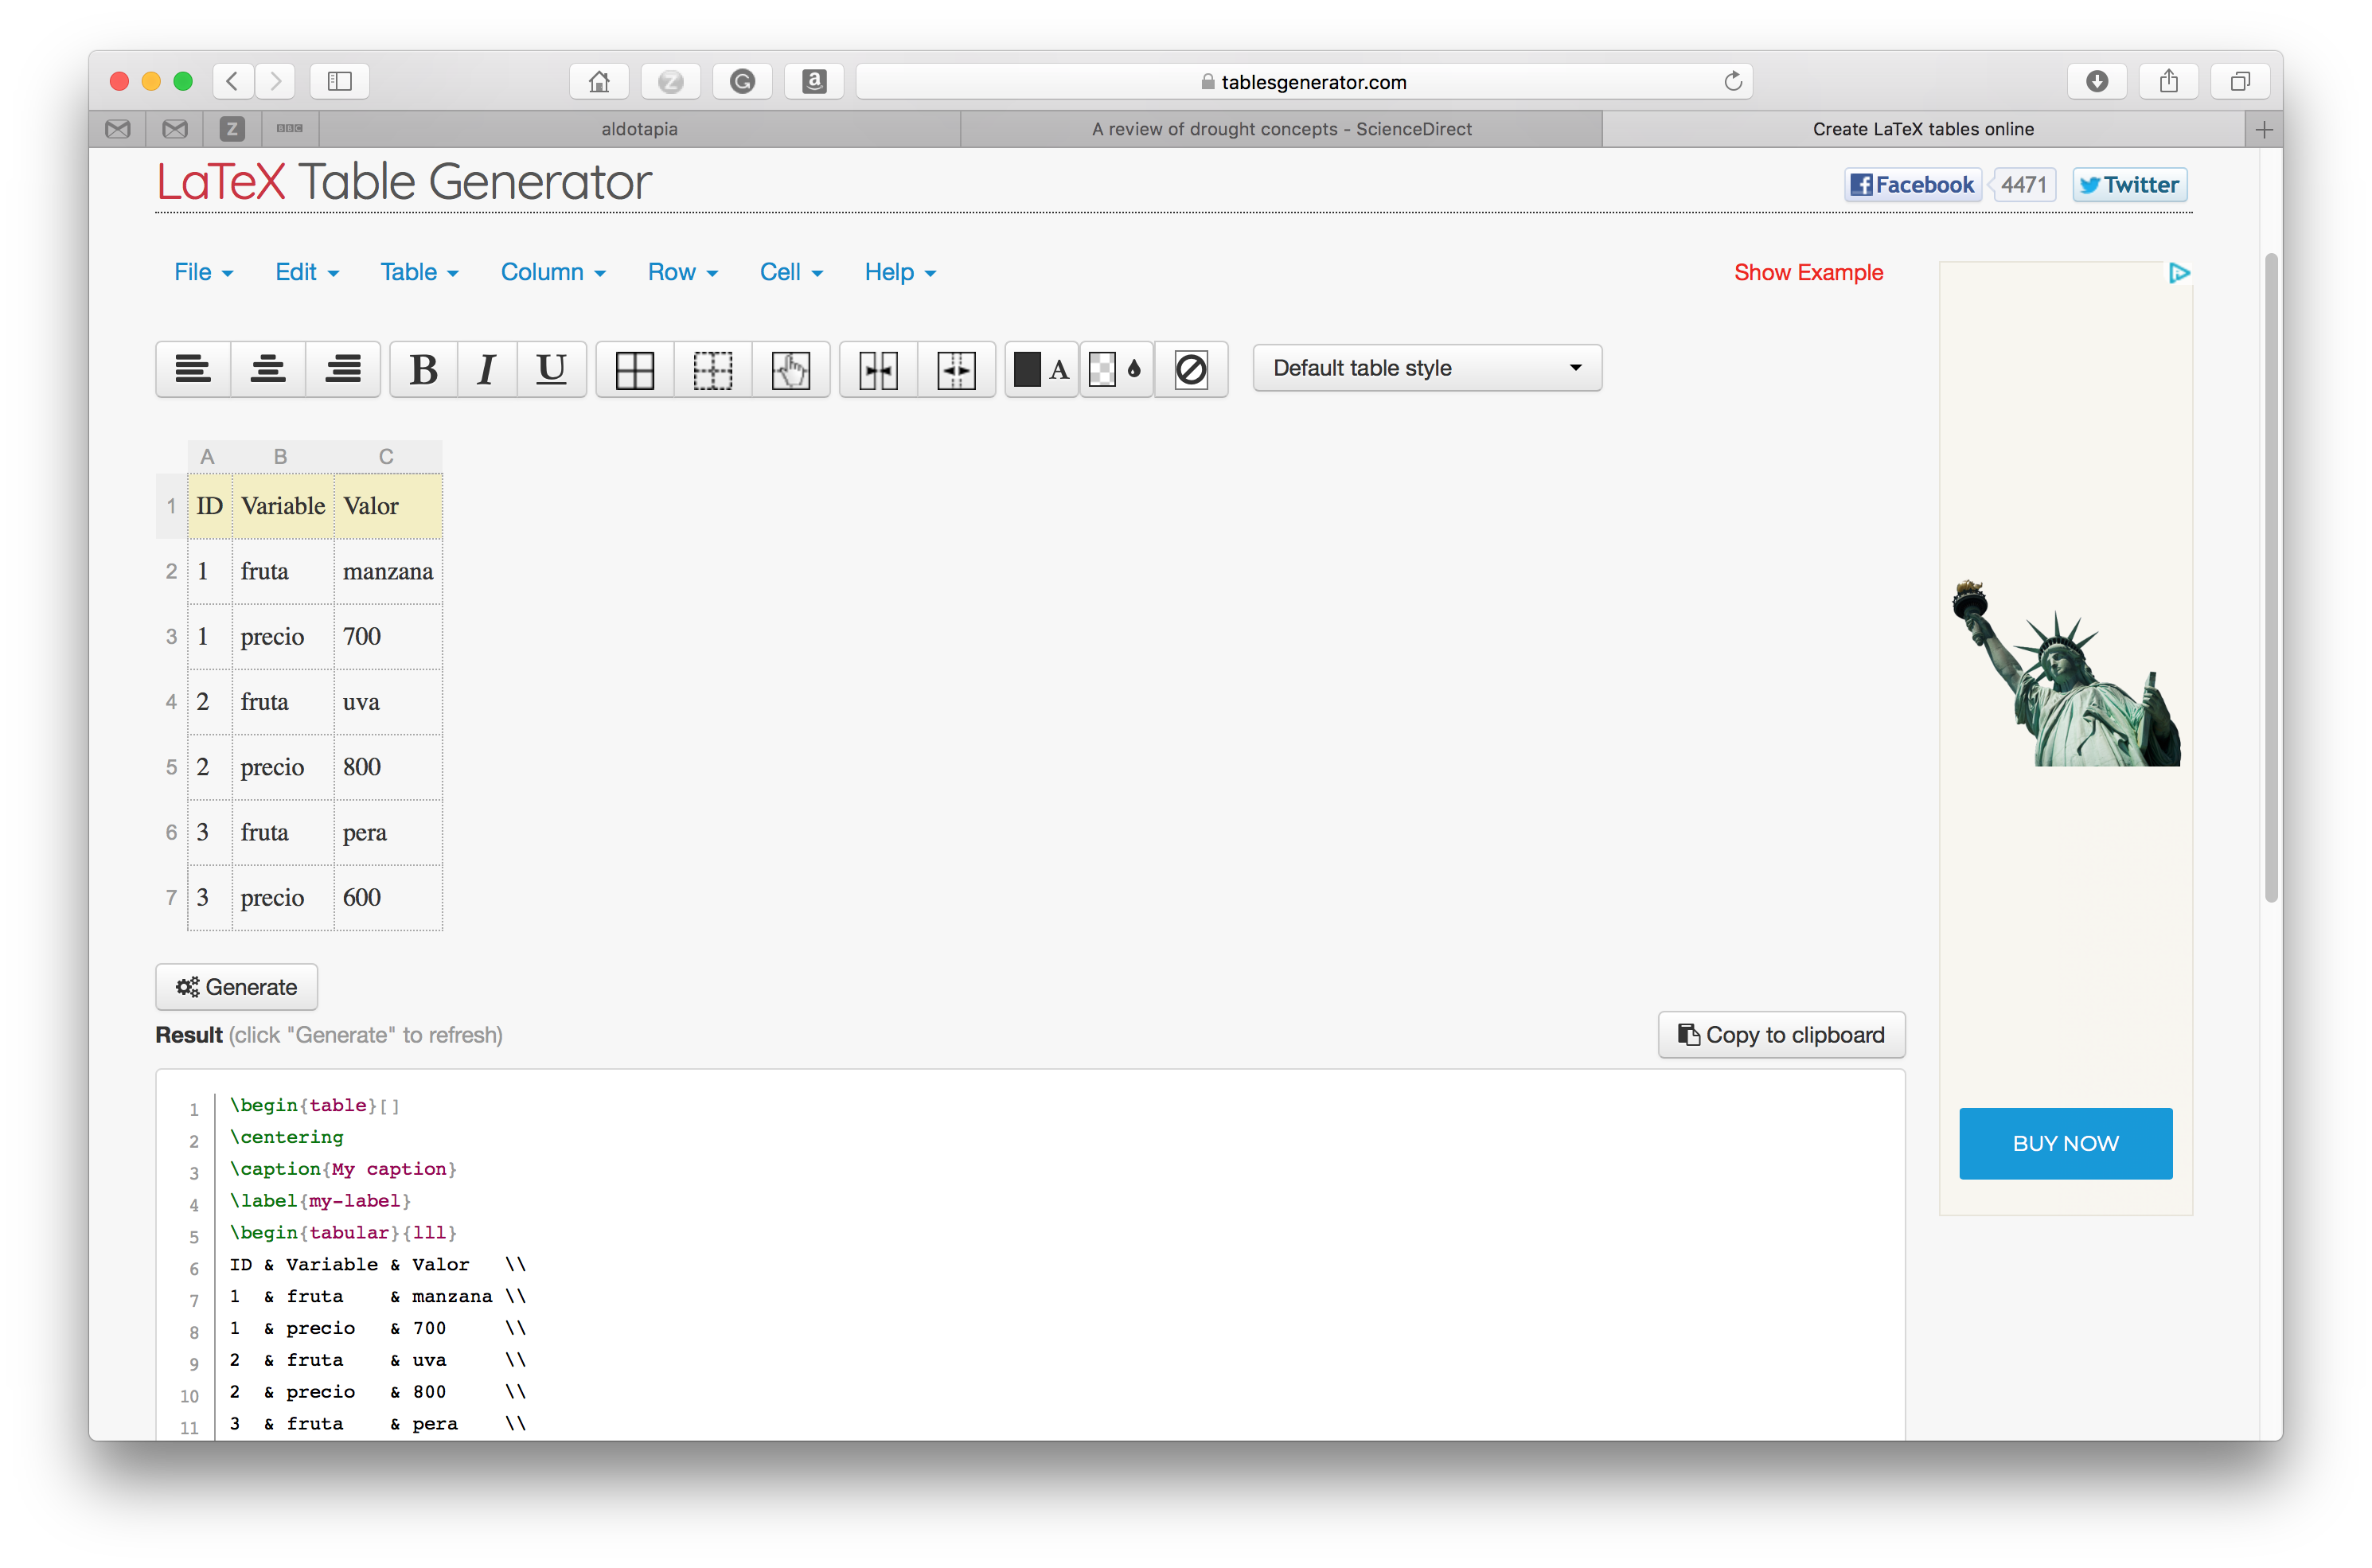
\includegraphics[width=\textwidth]{Figuras/tabla2.png}
\caption{Resultado}
\label{tabla2}
\end{center}
\end{figure}

\clearpage

\begin{table}[]
\centering
\caption{Descripción de la tabla}
\label{etiqueta_tabla}
\begin{tabular}{cll}
ID & Variable & Valor   \\
1  & fruta    & manzana \\
1  & precio   & 700     \\
2  & fruta    & uva     \\
2  & precio   & 800     \\
3  & fruta    & pera    \\
3  & precio   & 600    
\end{tabular}
\end{table}


\bibliographystyle{flexbib}
\bibliography{biblioteca.bib}


\end{document}  